\section{PLANIFICACIÓN DEL PROYECTO}
En este apartado se abordará la planificación inicial del proyecto, detallando los aspectos más relevantes del mismo. 
Se incluirá la identificación de interesados, las tareas a realizar, la estructura de desglose de trabajo, la planificación temporal, los riesgos identificados y el presupuesto inicial.

\subsection{Identificación de Interesados}
Los interesados en el proyecto son las personas o grupos que pueden afectar o verse afectados por el proyecto. En este caso, se identifican los siguientes interesados:
\begin{itemize}
    \item \textbf{Tutor del TFG:} Profesor de la Universidad de Oviedo encargado de la supervisión del proyecto.
    \item \textbf{Cliente:} Se entenderá como cliente la Universidad de Oviedo.
    \item \textbf{Equipo de Desarrollo:} En este caso, el equipo de desarrollo está formado por una única persona que es el alumno que realiza el TFG.
    \item \textbf{Usuarios:} Personas que utilizarán el producto final.
\end{itemize}

\subsection{OBS y PBS}
El OBS, \textit{Organizational Breakdown Structure} es una estructura que representa las responsabilidades sobre la realización de las tareas del proyecto. 
Por otro lado, el PBS (Product Breakdown Structure) es una estructura jerárquica que descompone el proyecto en los productos que se deben entregar para cumplir con los objetivos del proyecto.

\subsubsection{OBS}
En este proyecto, se simulará una pequeña empresa ficticia para su realización. 
Se han identificado los distintos perfiles que intervienen en el proyecto, así como las tareas que cada uno debe realizar. 
Aunque el proyecto se llevará a cabo de forma individual, se ha considerado necesario estructurar estos roles para poder asignar un presupuesto adecuado a cada función.

Los roles identificados se especifican en \coloredUnderline{\hyperlink{table:obs}{Tabla: \ref*{table:obs} \nameref*{table:obs}}}. 
Cabe destacar que el rol de Jefe de Proyecto (JP) es el encargado de supervisar y coordinar el trabajo de los demás roles y este rol ha sido considerado tanto para el alumno como para el tutor del TFG.


\begin{table}[H]
\centering
\hypertarget{table:obs}{}
\caption{OBS (Organizational Breakdown Structure)}
\label{table:obs}
\begin{tabular}{>{\columncolor{lightgreen!20}}p{7cm} p{10cm}}
\toprule
\rowcolor{darkgreen!50}
\textbf{Abreviatura} & \textbf{Rol} \\
\midrule
JP & Jefe de Proyecto \\
\midrule
AN & Analista junior\\
\midrule
DI & Diseñador junior \\
\midrule
DS & Desarrollador de Software junior\\
\midrule
TE & Tester junior \\
\midrule
DOC & Documentador técnico \\
\bottomrule
\end{tabular}
\end{table}
 
Se ha decidido realizar una matriz de asignación de responsabilidades RACI para relacionar las tareas identifcadas en \coloredUnderline{\hyperlink{sec:5-WBS}{\ref*{sec:5-WBS} \nameref*{sec:5-WBS}}} con cada rol.
En esta matriz, a cada tarea se le asigna un rol con una de las siguientes responsabilidades:
\begin{itemize}
    \item \textbf{R:} Responsable. Persona que realiza la tarea.
    \item \textbf{A:} Aprobador. Persona que aprueba la tarea.
    \item \textbf{C:} Consultado. Persona a la que se consulta sobre la tarea.
    \item \textbf{I:} Informado. Persona a la que se informa sobre el avance y los resultados de la tarea.
\end{itemize}
Un mismo recursos puede tener varias responsabilidades en una misma tarea, en tal caso se anotarán separadas por el caracter \textit{``/''}.

\subsubsubsection{Análisis del proyecto}
En la \coloredUnderline{\hyperlink{table:matriz-analisis}{Tabla: \ref*{table:matriz-analisis} \nameref*{table:matriz-analisis}}} se muestra la matriz de responsabilidades para la fase de análisis.
\begin{table}[H]
    \centering
    \caption{Matriz RACI. Análisis del proyecto}
    \label{table:matriz-analisis}
    \hypertarget{table:matriz-analisis}{}
    \begin{tabular}{
    >{\columncolor{lightgreen!20}}m{7cm} 
    >{\columncolor{white}}m{1cm} 
    >{\columncolor{white}}m{1cm} 
    >{\columncolor{white}}m{1cm} 
    >{\columncolor{white}}m{1cm} 
    >{\columncolor{white}}m{1cm} 
    >{\columncolor{white}}m{1cm}}
    \cmidrule(l){2-7}
    \rowcolor{darkgreen!50}
    \cellcolor{white} & \multicolumn{6}{c}{\textbf{Roles}} \\
    \midrule
    \rowcolor{lightgreen!20}
    \cellcolor{darkgreen!50}\textbf{Tarea} & \textbf{JP} & \textbf{AN} & \textbf{DI} & \textbf{DS} & \textbf{TE} & \textbf{DOC} \\
    \midrule
    Análisis del sistema & A & R &  & C &  &  \\
    \midrule
    Análisis de la arquitectura & A & R &  & C &  &  \\
    \midrule
    Análisis de la infraestructura & A & R &  & C &  &  \\
    \midrule
    Determinación del alcance de desarrollo & A & R & I & C & I & I \\
    \bottomrule
    \end{tabular}
\end{table}

\subsubsubsection{Seguimiento del proyecto}
En la \coloredUnderline{\hyperlink{table:matriz-seguimiento}{Tabla: \ref*{table:matriz-seguimiento} \nameref*{table:matriz-seguimiento}}} se muestra la matriz de responsabilidades para la fase de seguimiento.
\begin{table}[H]
    \centering
    \caption{Matriz RACI. Seguimiento del proyecto}
    \label{table:matriz-seguimiento}
    \hypertarget{table:matriz-seguimiento}{}
    \begin{tabular}{
    >{\columncolor{lightgreen!20}}m{7cm} 
    >{\columncolor{white}}m{1cm} 
    >{\columncolor{white}}m{1cm} 
    >{\columncolor{white}}m{1cm} 
    >{\columncolor{white}}m{1cm} 
    >{\columncolor{white}}m{1cm} 
    >{\columncolor{white}}m{1cm}}
    \cmidrule(l){2-7}
    \rowcolor{darkgreen!50}
    \cellcolor{white} & \multicolumn{6}{c}{\textbf{Roles}} \\
    \midrule
    \rowcolor{lightgreen!20}
    \cellcolor{darkgreen!50}\textbf{Tarea} & \textbf{JP} & \textbf{AN} & \textbf{DI} & \textbf{DS} & \textbf{TE} & \textbf{DOC} \\
    \midrule
    Reunión de arranque & A & I & I & I & I & R \\
    \midrule
    Reuniones periódicas & A & I & I & I & I & R\\
    \midrule
    Reunión de revisión & A & I & I & C & I & R  \\
    \midrule
    Reunión final & A & I & I & C & I & R  \\
    \bottomrule
    \end{tabular}
\end{table}

\subsubsubsection{Diseño del sistema}
En la \coloredUnderline{\hyperlink{table:matriz-diseno}{Tabla: \ref*{table:matriz-diseno} \nameref*{table:matriz-diseno}}} se presenta la matriz de responsabilidades correspondiente a la fase de diseño. 
Las tareas listadas en esta matriz son las tareas "hoja" de dicha fase, es decir, aquellas que no se descomponen en subtareas más pequeñas y, por lo tanto, representan las tareas finales 
de la fase de diseño.
\begin{table}[H]
    \centering
    \caption{Matriz RACI. Diseño del sistema}
    \label{table:matriz-diseno}
    \hypertarget{table:matriz-diseno}{}
    \begin{tabular}{
    >{\columncolor{lightgreen!20}}m{7cm} 
    >{\columncolor{white}}m{1cm} 
    >{\columncolor{white}}m{1cm} 
    >{\columncolor{white}}m{1cm} 
    >{\columncolor{white}}m{1cm} 
    >{\columncolor{white}}m{1cm} 
    >{\columncolor{white}}m{1cm}}
    \cmidrule(l){2-7}
    \rowcolor{darkgreen!50}
    \cellcolor{white} & \multicolumn{6}{c}{\textbf{Roles}} \\
    \midrule
    \rowcolor{lightgreen!20}
    \cellcolor{darkgreen!50}\textbf{Tarea} & \textbf{JP} & \textbf{AN} & \textbf{DI} & \textbf{DS} & \textbf{TE} & \textbf{DOC} \\
    \midrule
    \textit{Backend}. Diseño del módulo de usuarios & A &  & I & R &  &  I \\
    \midrule
    \textit{Backend}. Diseño del módulo de cartas & A &  & I & R &  & I \\
    \midrule
    \textit{Backend}. Diseño del módulo de sobres de cartas & A &  & I & R &  & I \\
    \midrule
    \textit{Backend}. Diseño del módulo de subastas & A &  & I & R &  & I \\
    \midrule
    \textit{Backend}. Diseño del módulo de transacciones & A &  & I & R &  & I \\
    \midrule
    \textit{Frontend}. Diseño de logo de la aplicación & A &  & R & I &  & I \\
    \midrule
    \textit{Frontend}. Diseño de la moneda de la aplicación & A &  & R & I &  & I \\
    \midrule
    \textit{Frontend}. Diseño de la temática & A &  & R & C/I &  & I \\
    \midrule
    \textit{Frontend}. Diseño del árbol de navegación & A &  & R & C/I &  & I \\
    \midrule
    \textit{Frontend}. Diseño de las páginas de información & A &  & R & C/I &  & I \\
    \midrule
    \textit{Frontend}. Diseño de las página \textit{Home} & A &  & R & C/I &  & I \\
    \midrule
    \textit{Frontend}. Diseño de las página de error & A &  & R & C/I &  & I \\
    \bottomrule
    \end{tabular}
\end{table}

\subsubsubsection{Implementación del sistema}
En la \coloredUnderline{\hyperlink{table:matriz-implementacion}{Tabla: \ref*{table:matriz-implementacion} \nameref*{table:matriz-implementacion}}} se muestra la matriz de responsabilidades para la fase de implementación.
\begin{table}[H]
    \centering
    \caption{Matriz RACI. Implementación del proyecto}
    \label{table:matriz-implementacion}
    \hypertarget{table:matriz-implementacion}{}
    \begin{tabular}{
    >{\columncolor{lightgreen!20}}m{7cm} 
    >{\columncolor{white}}m{1cm} 
    >{\columncolor{white}}m{1cm} 
    >{\columncolor{white}}m{1cm} 
    >{\columncolor{white}}m{1cm} 
    >{\columncolor{white}}m{1cm} 
    >{\columncolor{white}}m{1cm}}
    \cmidrule(l){2-7}
    \rowcolor{darkgreen!50}
    \cellcolor{white} & \multicolumn{6}{c}{\textbf{Roles}} \\
    \midrule
    \rowcolor{lightgreen!20}
    \cellcolor{darkgreen!50}\textbf{Tarea} & \textbf{JP} & \textbf{AN} & \textbf{DI} & \textbf{DS} & \textbf{TE} & \textbf{DOC} \\
    \midrule
    Reunión de arranque & A & I & I & I & I & R \\
    \midrule
    Reuniones periódicas & A & I & I & I & I & R\\
    \midrule
    Reunión de revisión & A & I & I & C & I & R  \\
    \midrule
    Reunión final & A & I & I & C & I & R  \\
    \bottomrule
    \end{tabular}
\end{table}

\subsubsection{PBS}
El PBS, \textit{Product Breakdown Structure}, es una estructura jerárquica que descompone el proyecto en los productos que se deben entregar para cumplir 
con los objetivos del proyecto. 
En las siguientes secciones se detallan los productos que se deben entregar en el proyecto BidMon Universe.

\subsubsection{PBS. Visión general}
En la \coloredUnderline{\hyperlink{fig:5_PBS-Vision-General}{Figura \ref*{fig:5_PBS-Vision-General}: \nameref*{fig:5_PBS-Vision-General}}} se muestran los productos de alto nivel que se deben entregar en el proyecto BidMon Universe. 
En las siguientes secciones, se entrará en detalle en cada uno de los productos.

\begin{figure}[H]
    \hypertarget{fig:5_PBS-Vision-General}{}
    \centering
    \includegraphics[width=0.5\linewidth]{figures/5-PBS/5_PBS-Vision-General.png}
    \caption{PBS. Visión general}
    \label{fig:5_PBS-Vision-General}
\end{figure}


\subsubsection{PBS. Análisis del sistema}
En la \coloredUnderline{\hyperlink{fig:5_PBS-Analisis-Sistema}{Figura \ref*{fig:5_PBS-Analisis-Sistema}: \nameref*{fig:5_PBS-Analisis-Sistema}}}, se detallan los productos que se deben entregar en la fase de análisis del sistema.
\begin{figure}[H]
    \hypertarget{fig:5_PBS-Analisis-Sistema}{}
    \centering
    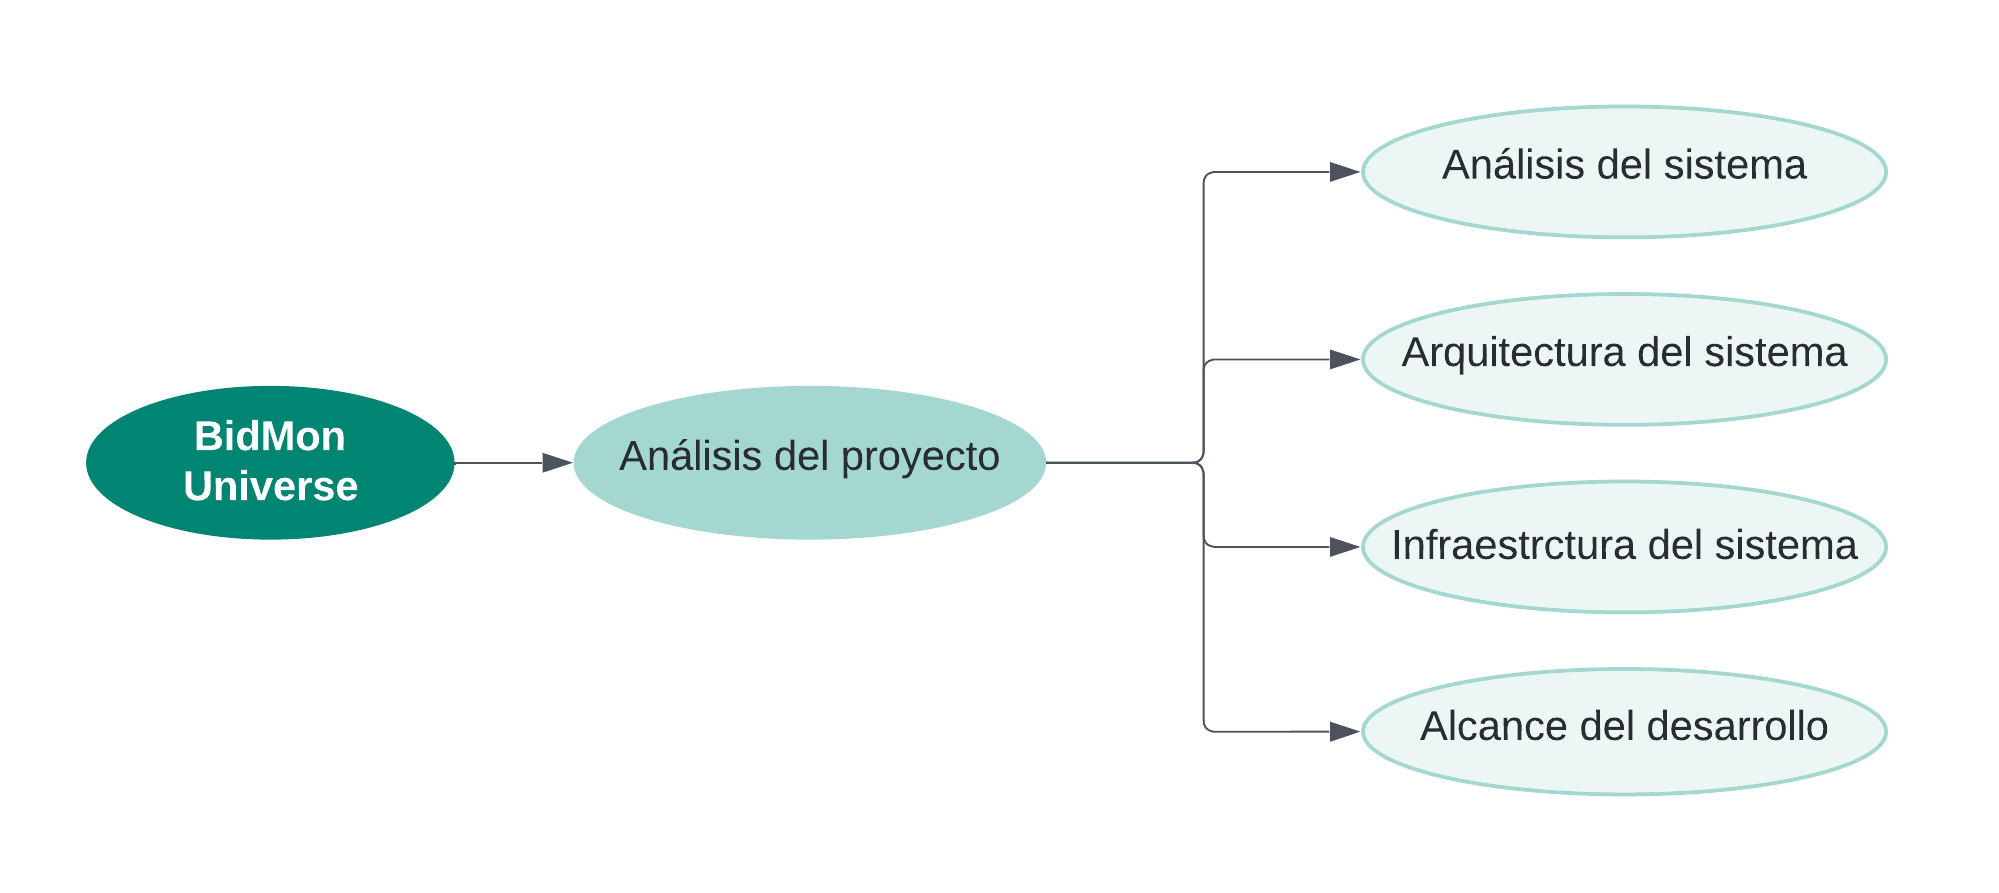
\includegraphics[width=0.7\linewidth]{figures/5-PBS/5_PBS-Analisis.png}
    \caption{PBS. Análisis del sistema}
    \label{fig:5_PBS-Analisis-Sistema}
\end{figure}

\subsubsection{PBS. Seguimiento del sistema}
En esta fase se detallan los productos que se obtienen en la fase de segumiento del proyecto, principalmente documentación e informes como se muestra en la \coloredUnderline{\hyperlink{fig:5_PBS-Seguimiento-Sistema}{Figura \ref*{fig:5_PBS-Seguimiento-Sistema}: \nameref*{fig:5_PBS-Seguimiento-Sistema}}}.
\begin{figure}[H]
    \hypertarget{fig:5_PBS-Seguimiento-Sistema}{}
    \centering
    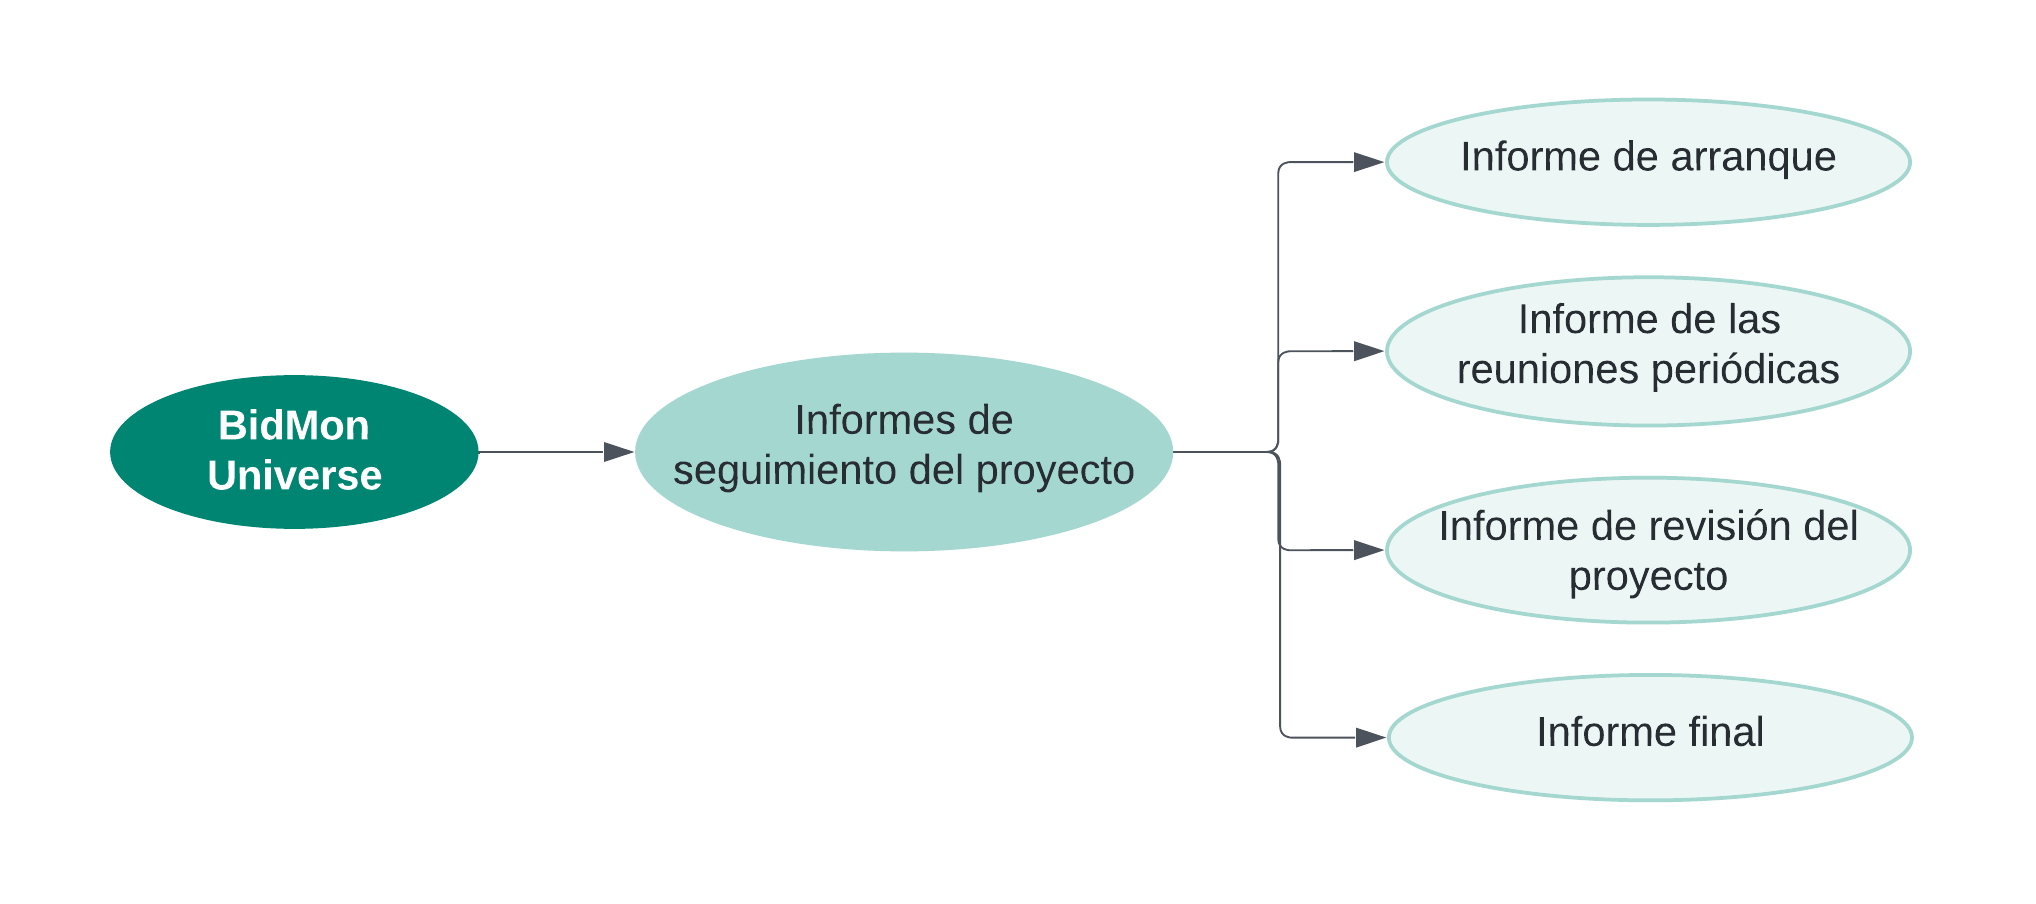
\includegraphics[width=0.7\linewidth]{figures/5-PBS/5_PBS-Seguimiento.png}
    \caption{PBS. Seguimiento del sistema}
    \label{fig:5_PBS-Seguimiento-Sistema}
\end{figure}

\subsubsection{PBS. Diseño del sistema}
En la \coloredUnderline{\hyperlink{fig:5_PBS-Diseño-Sistema}{Figura \ref*{fig:5_PBS-Diseño-Sistema}: \nameref*{fig:5_PBS-Diseño-Sistema}}}, se detallan los productos que se deben entregar en la fase de diseño del sistema.
\begin{figure}[H]
    \hypertarget{fig:5_PBS-Diseño-Sistema}{}
    \centering
    \includegraphics[width=0.9\linewidth]{figures/5-PBS/5_PBS-Diseno.png}
    \caption{PBS. Diseño del sistema}
    \label{fig:5_PBS-Diseño-Sistema}
\end{figure}

\subsubsection{PBS. Implementación del sistema}
En la \coloredUnderline{\hyperlink{fig:5_PBS-Implementación-Sistema}{Figura \ref*{fig:5_PBS-Implementación-Sistema}: \nameref*{fig:5_PBS-Implementación-Sistema}}}, se detallan los productos a realizar en la fase de implementación del sistema.
\begin{figure}[H]
    \hypertarget{fig:5_PBS-Implementación-Sistema}{}
    \centering
    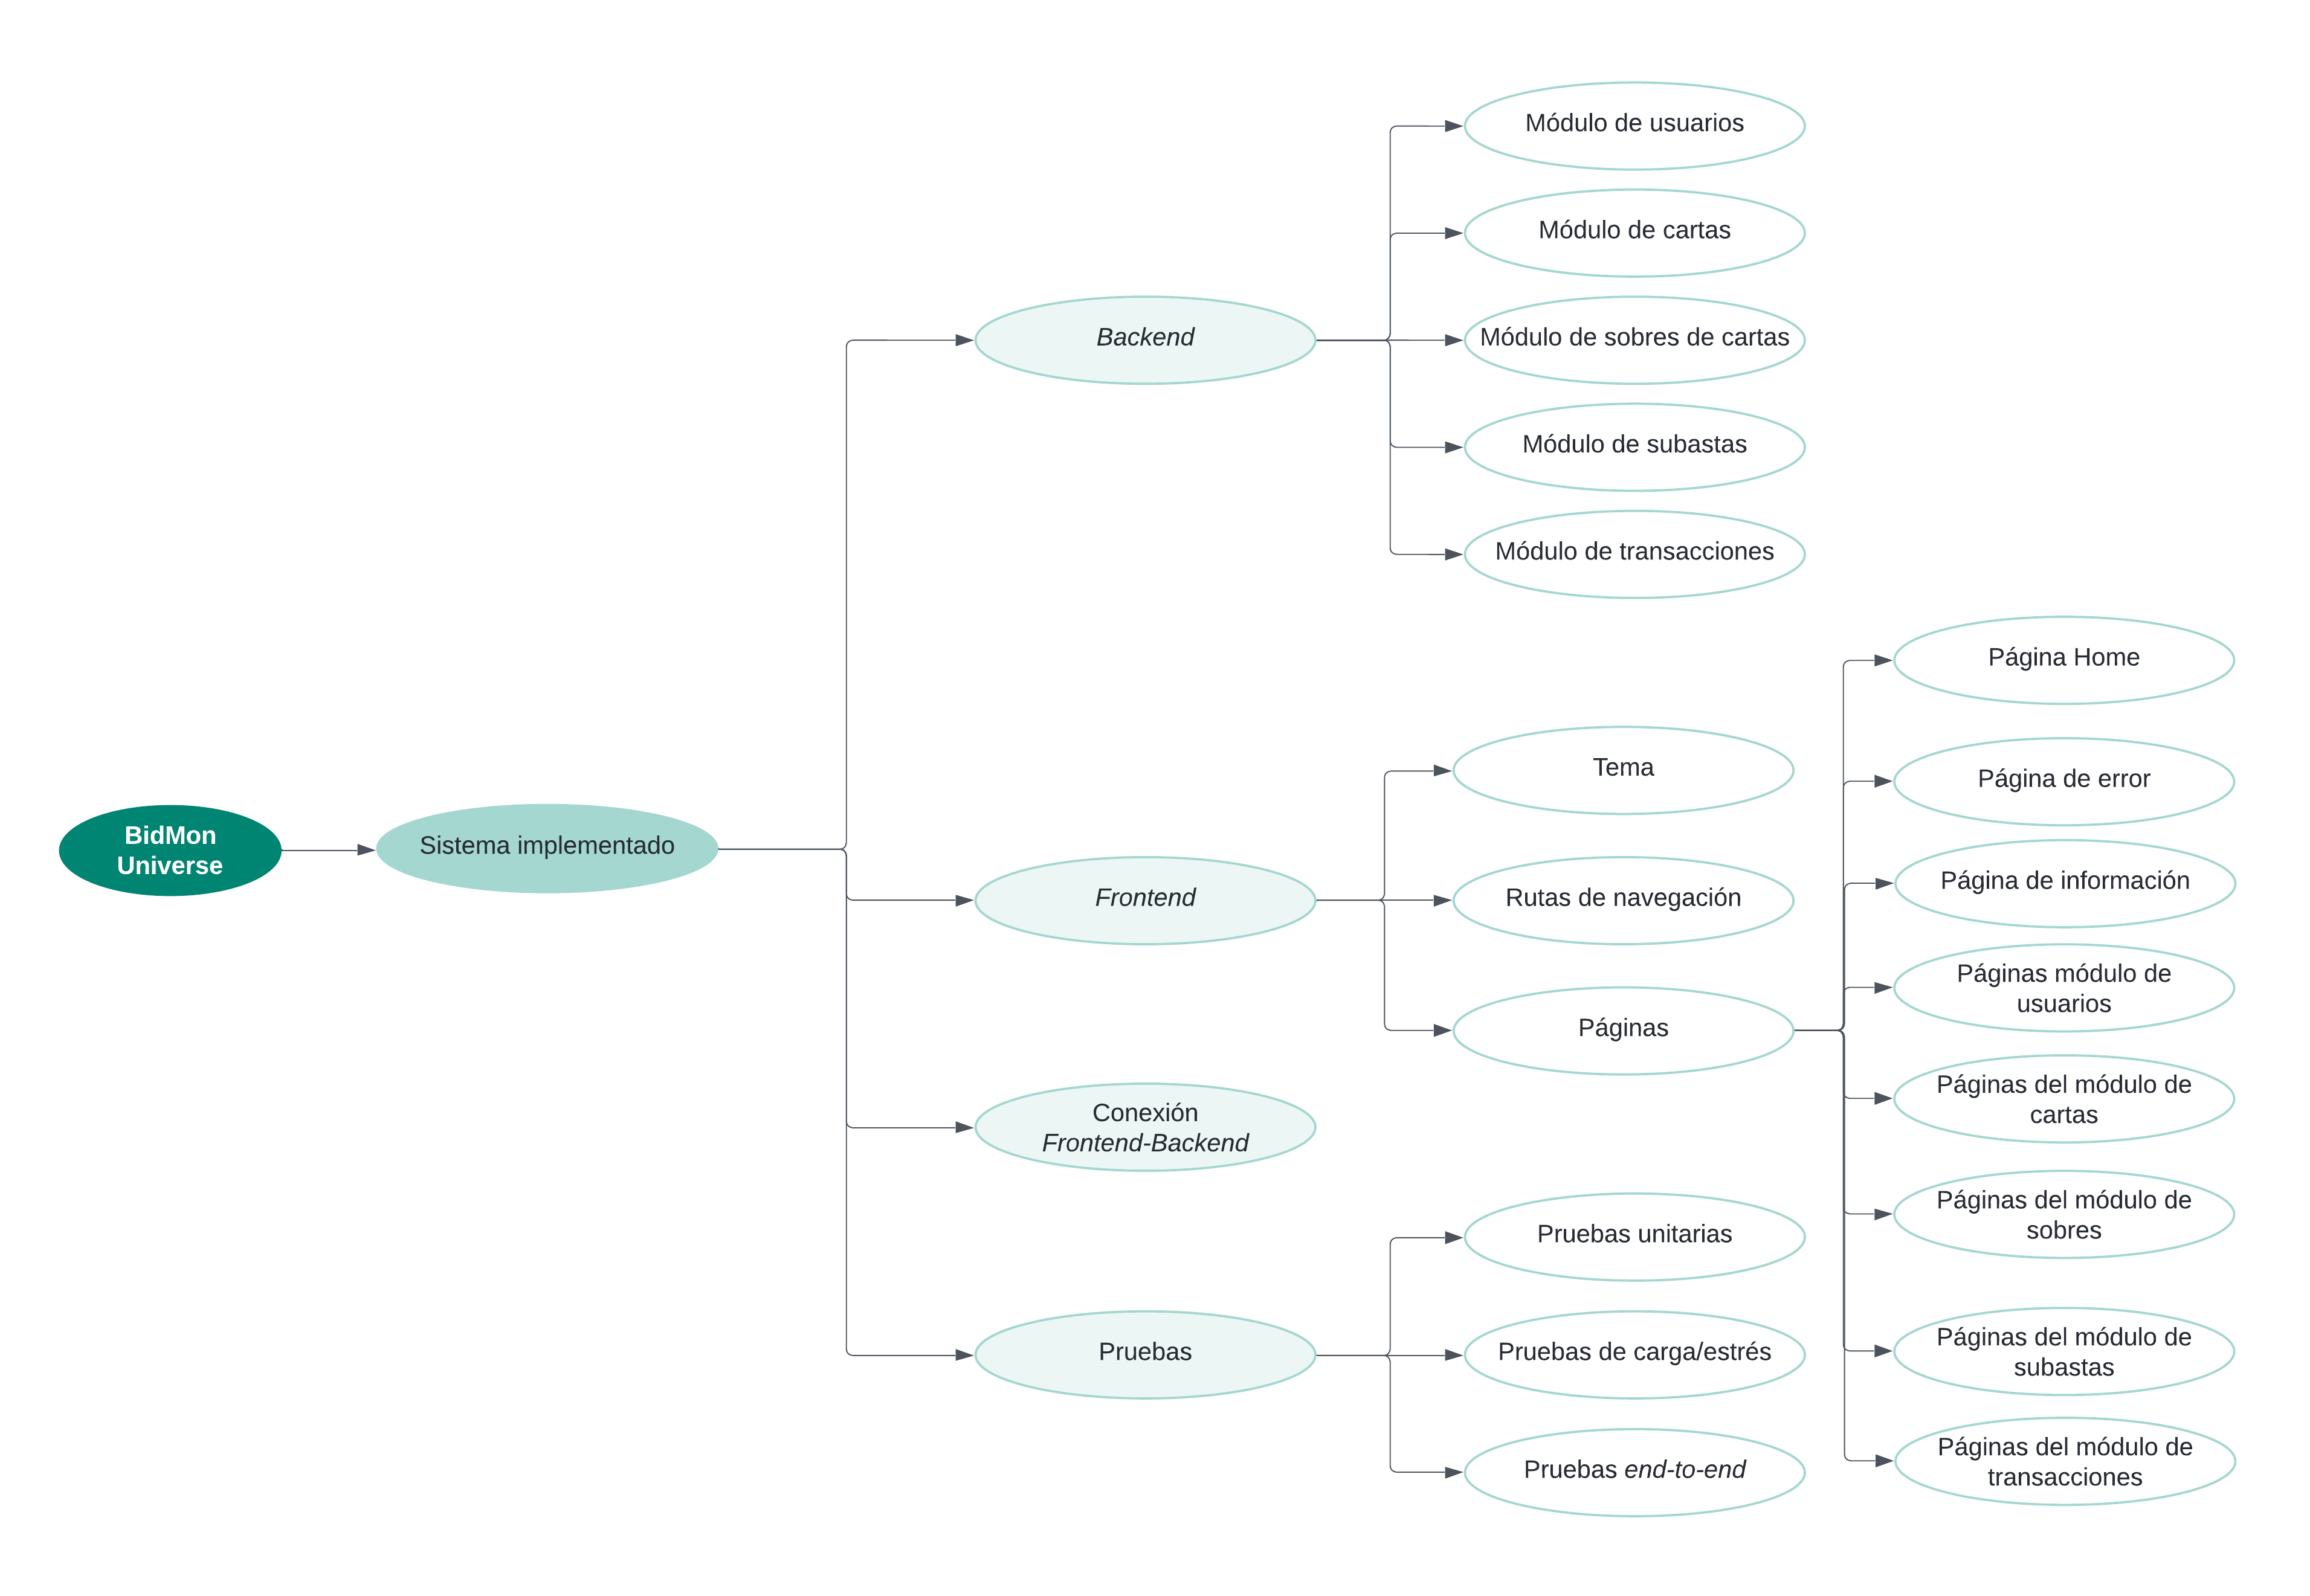
\includegraphics[width=0.9\linewidth]{figures/5-PBS/5_PBS-Implementacion.png}
    \caption{PBS. Implementación del sistema}
    \label{fig:5_PBS-Implementación-Sistema}
\end{figure}

\subsubsection{PBS. Pruebas del sistema}
En la fase de pruebas del sistema se obtienen como productos los resultados de la ejecución de dichas pruebas.
\begin{figure}[H]
    \hypertarget{fig:5_PBS-Pruebas-Sistema}{}
    \centering
    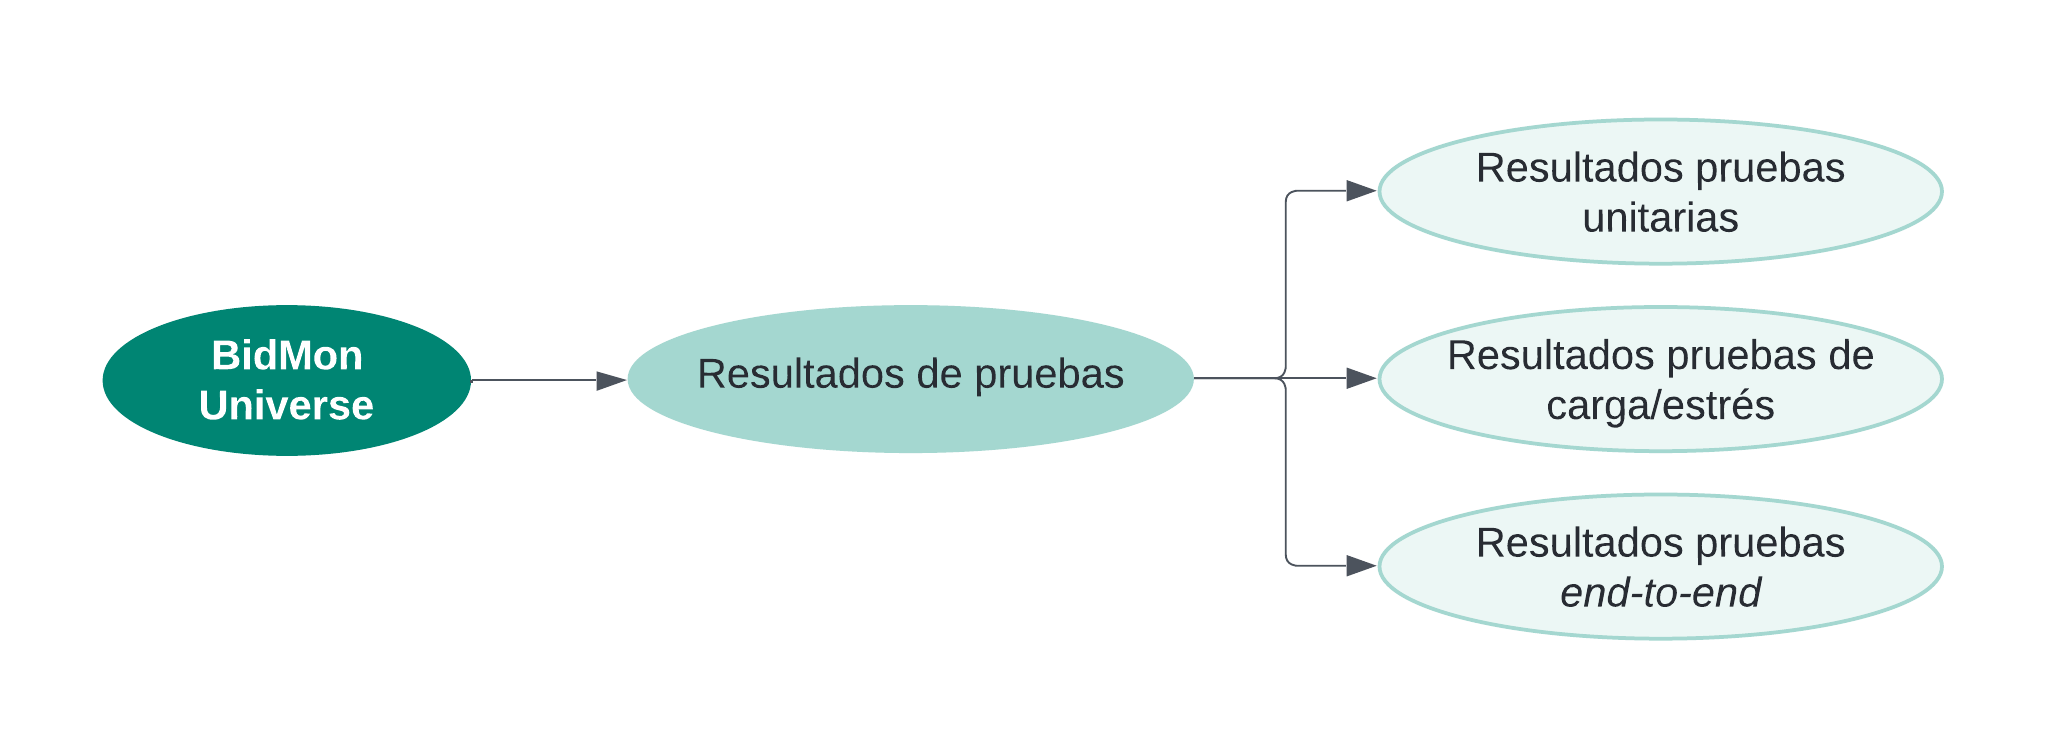
\includegraphics[width=0.7\linewidth]{figures/5-PBS/5_PBS-Pruebas.png}
    \caption{PBS. Pruebas del sistema}
    \label{fig:5_PBS-Pruebas-Sistema}
\end{figure}

\subsubsection{PBS. Despliegue del sistema}
En la fase de despliegue del sistema se obtiene como producto el sistema desplegado y en funcionamiento.
\begin{figure}[H]
    \hypertarget{fig:5_PBS-Despliegue-Sistema}{}
    \centering
    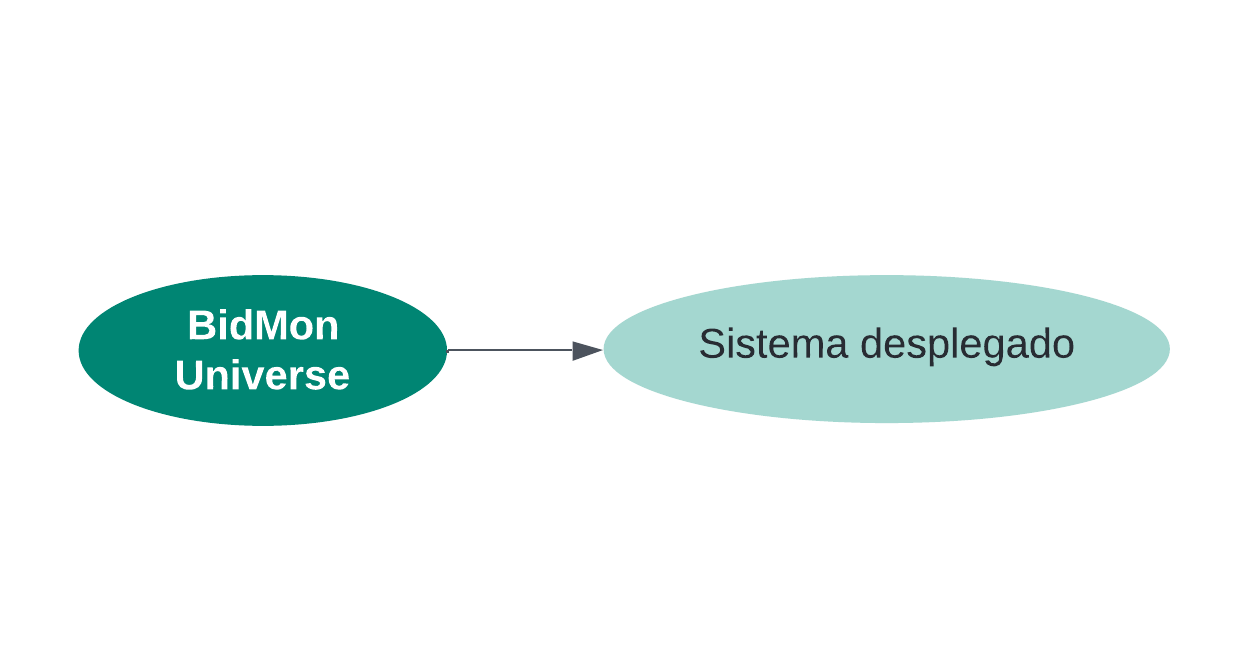
\includegraphics[width=0.7\linewidth]{figures/5-PBS/5_PBS-Despliegue.png}
    \caption{PBS. Despliegue del sistema}
    \label{fig:5_PBS-Despliegue-Sistema}
\end{figure}


\subsubsection{PBS. Documentación del sistema}
En la fase de documentación del sistema se obtienen como productos los documentos técnicos que describen el proyecto junto con los anexos.
\begin{figure}[H]
    \hypertarget{fig:5_PBS-Documentación-Sistema}{}
    \centering
    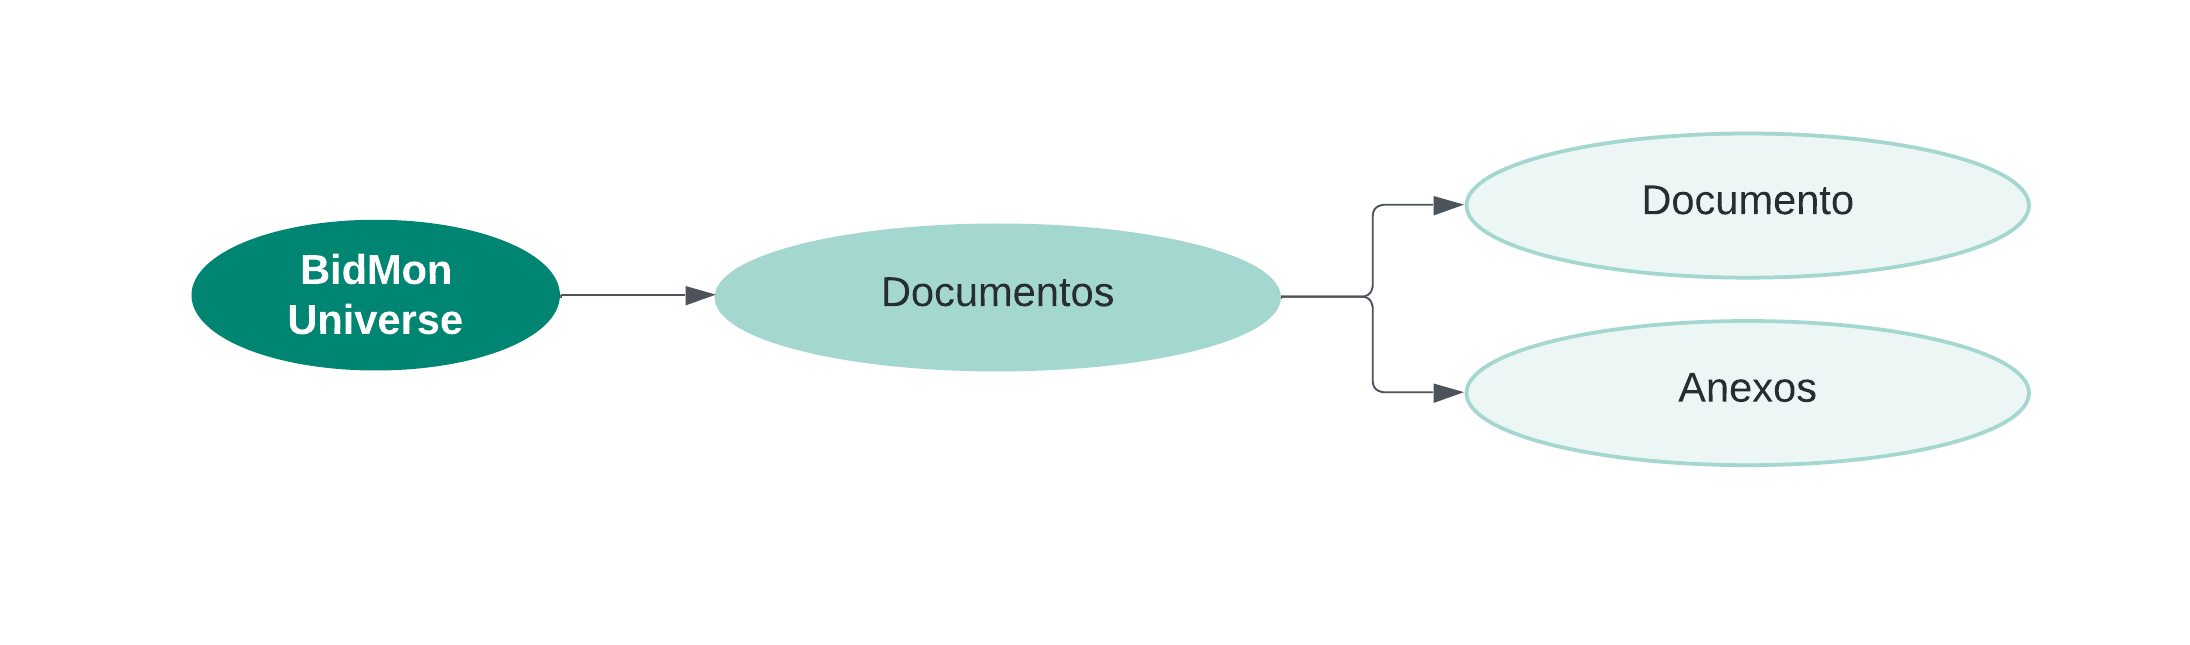
\includegraphics[width=0.7\linewidth]{figures/5-PBS/5_PBS-Documento.png}
    \caption{PBS. Documentación del sistema}
    \label{fig:5_PBS-Documentación-Sistema}
\end{figure}



\subsection{Planificación Inicial. WBS}
\subsubsection{WBS}
En esta sección se detalla la estructura de desglose del trabajo del proyecto también conocida como WBS, \textit{Work Breakdown Structure}. 
En ella se especifican las tareas necesarias para obtener los productos detallados en \coloredUnderline{\hyperlink{sec:5-PBS}{\ref*{sec:5-PBS} \nameref*{sec:5-PBS}}}.

Estas tareas se representan en forma de árbol jerárquico, donde cada rama representa una tarea y sus subramas las tareas que la componen.
El diagrama se ha dividido en las fases en las que se divide el proyecto para mejorar la legibilidad, facilitando la comprensión de las tareas y sub-tareas que se deben realizar en cada una de ellas.

\subsubsubsection{WBS. Visión general}
En la \coloredUnderline{\hyperlink{fig:5_WBS-Vision-General}{Figura \ref*{fig:5_WBS-Vision-General}: \nameref*{fig:5_WBS-Vision-General}}} se muestra la estructura de desglose del trabajo del proyecto de alto nivel, es decir, 
las tareas generales o fases que se deben realizar para cumplir con los objetivos del proyecto.
En las siguientes secciones, se entrará en detalle en cada una de las tareas.
\begin{figure}[H]
    \hypertarget{fig:5_WBS-Vision-General}{}
    \centering
    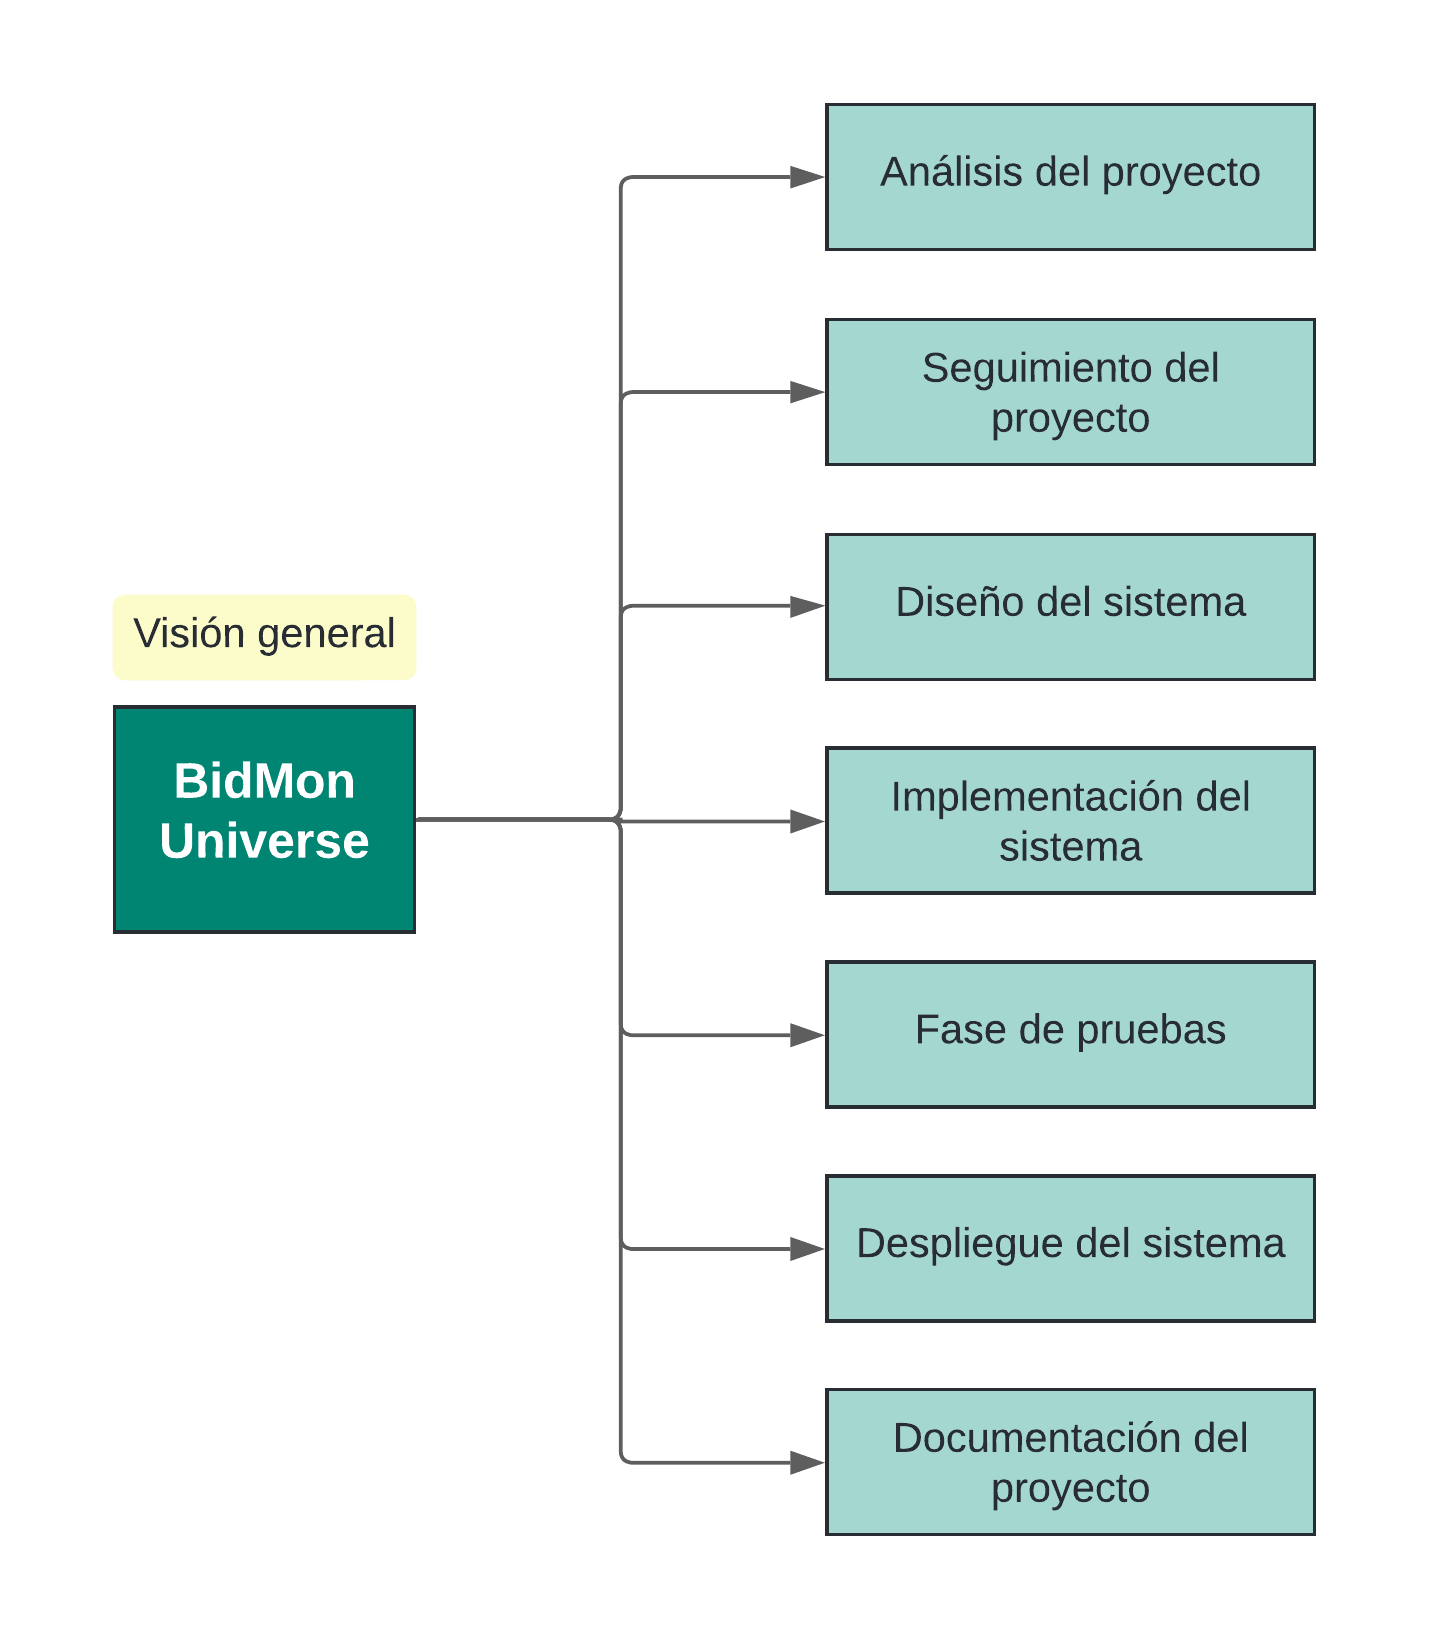
\includegraphics[width=0.5\linewidth]{figures/5-WBS/5_WBS-Vision-General.png}
    \caption{WBS. Visión general}
    \label{fig:5_WBS-Vision-General}
\end{figure}

\subsubsubsection{WBS. Análisis del proyecto}
En la \coloredUnderline{\hyperlink{fig:5_WBS-Analisis}{Figura \ref*{fig:5_WBS-Analisis}: \nameref*{fig:5_WBS-Analisis}}}, se detallan las tareas que se deben realizar en la fase de análisis del sistema para cumplir con los objetivos del proyecto.
\begin{figure}[H]
    \hypertarget{fig:5_WBS-Analisis}{}
    \centering
    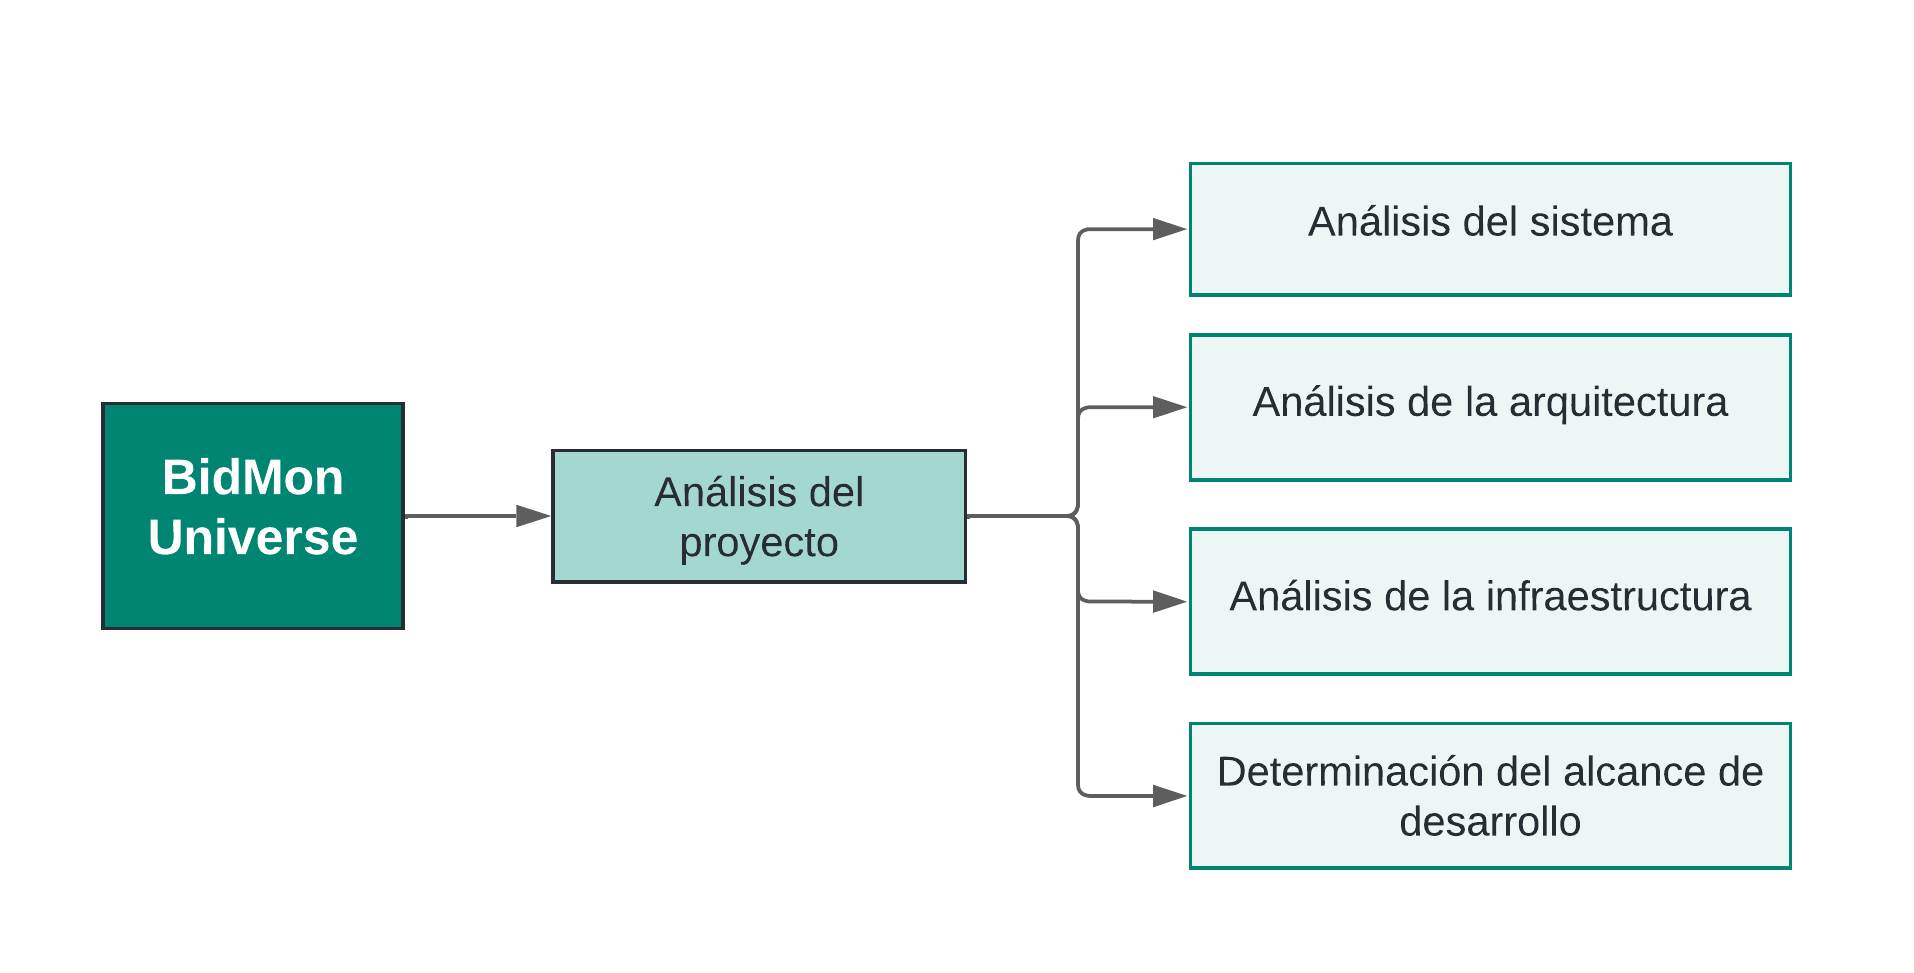
\includegraphics[width=0.7\linewidth]{figures/5-WBS/5_WBS-Analisis.png}
    \caption{WBS. Análisis del proyecto}
    \label{fig:5_WBS-Analisis}
\end{figure}

\subsubsubsection{WBS. Seguimiento del sistema}
En esta fase se realizan las tareas de seguimiento del proyecto, a través de distintas reuniones en las que se recopilará infomarción sobre el avance del proyecto. 
\begin{figure}[H]
    \hypertarget{fig:5_WBS-Seguimiento}{}
    \centering
    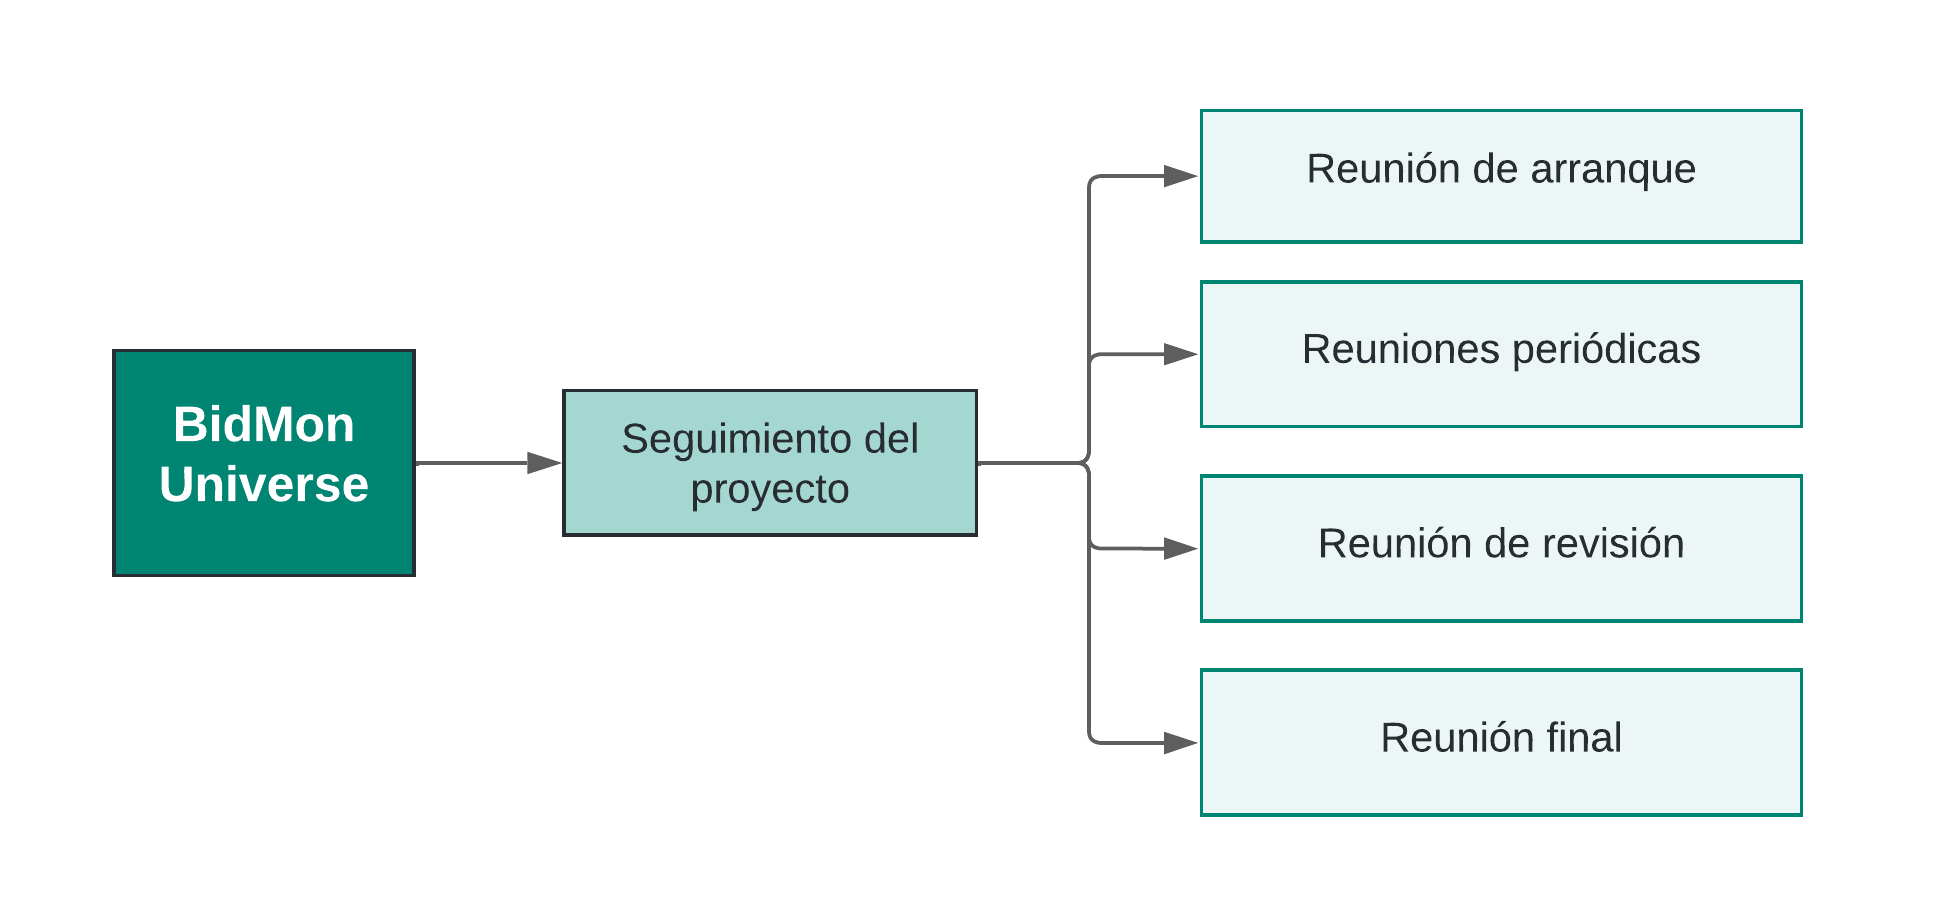
\includegraphics[width=0.7\linewidth]{figures/5-WBS/5_WBS-Seguimiento.png}
    \caption{WBS. Seguimiento del sistema}
    \label{fig:5_WBS-Seguimiento}
\end{figure}

\subsubsubsection{WBS. Diseño del sistema}
En la \coloredUnderline{\hyperlink{fig:5_WBS-Diseno}{Figura \ref*{fig:5_WBS-Diseno}: \nameref*{fig:5_WBS-Diseno}}}, se detallan las tareas que se deben realizar en la fase de diseño del sistema.
\begin{figure}[H]
    \hypertarget{fig:5_WBS-Diseno}{}
    \centering
    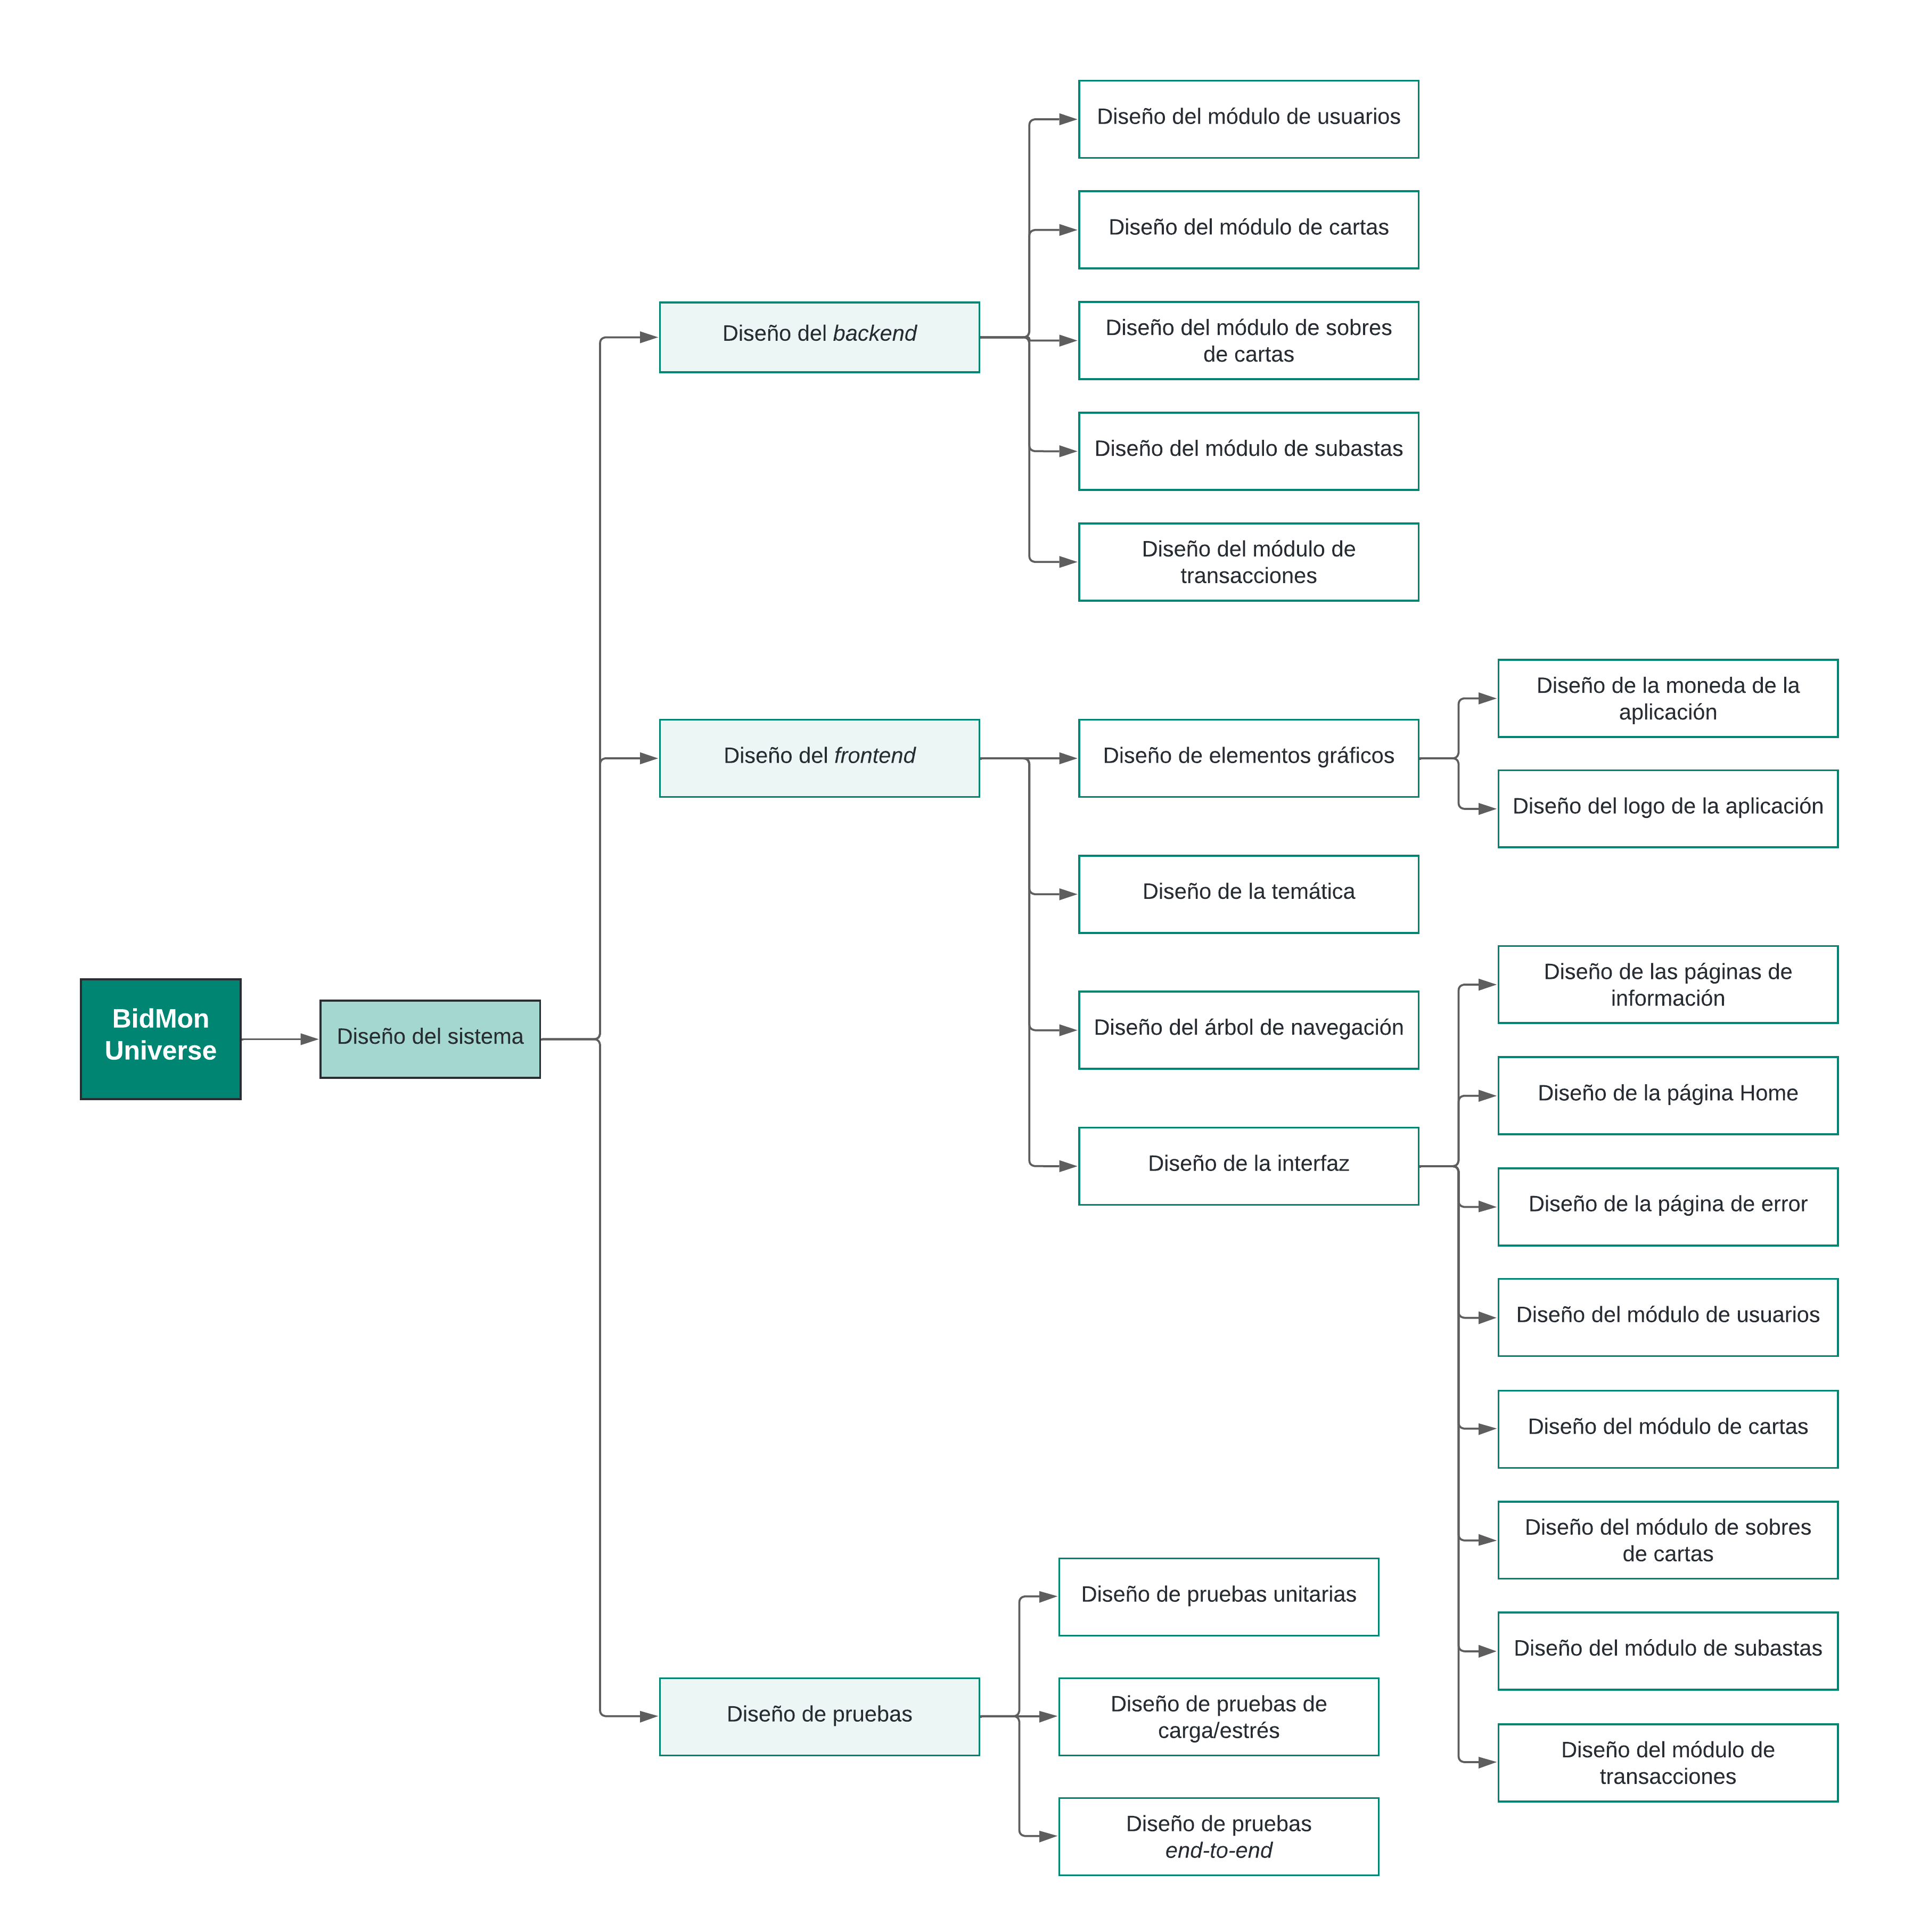
\includegraphics[width=0.9\linewidth]{figures/5-WBS/5_WBS-Diseno.png}
    \caption{WBS. Diseño del sistema}
    \label{fig:5_WBS-Diseno}
\end{figure}

\subsubsubsection{WBS. Implementación del sistema}
En la \coloredUnderline{\hyperlink{fig:5_WBS-Implementacion}{Figura \ref*{fig:5_WBS-Implementacion}: \nameref*{fig:5_WBS-Implementacion}}}, se detallan las tareas que se deben realizar en la fase de implementación del sistema.
\begin{figure}[H]
    \hypertarget{fig:5_WBS-Implementacion}{}
    \centering
    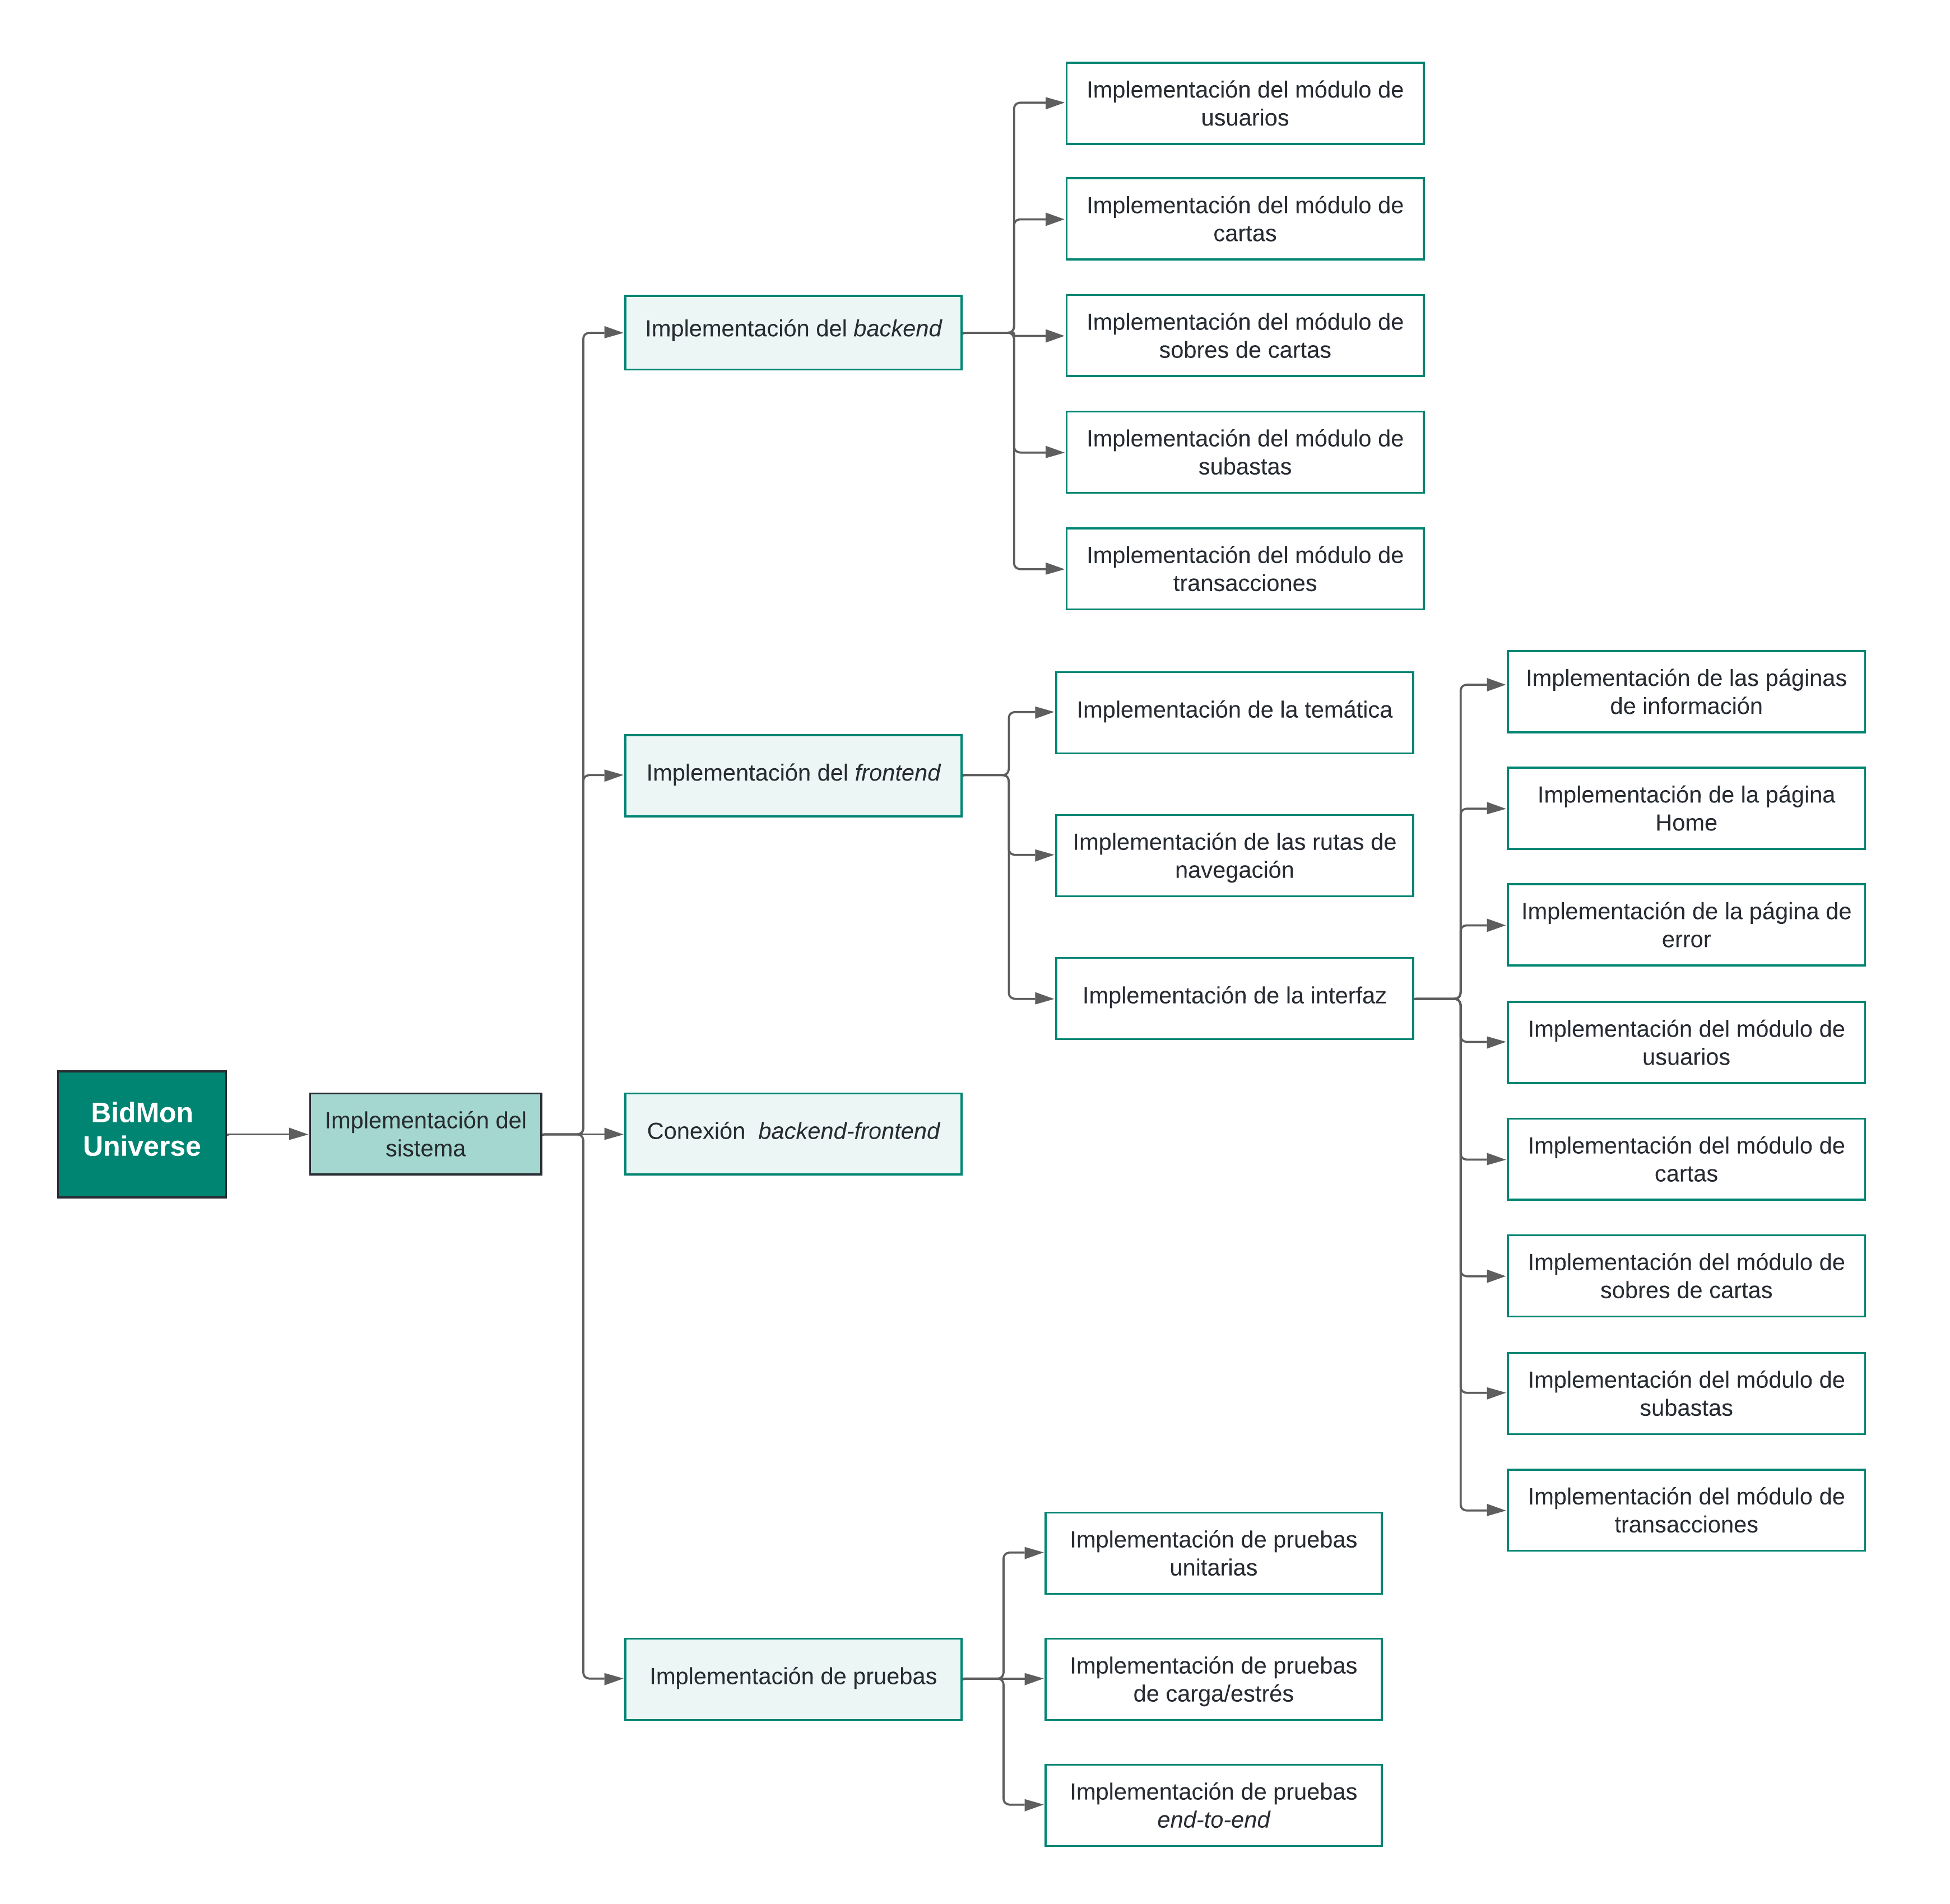
\includegraphics[width=0.9\linewidth]{figures/5-WBS/5_WBS-Implementacion.png}
    \caption{WBS. Implementación del sistema}
    \label{fig:5_WBS-Implementacion}
\end{figure}

\subsubsubsection{WBS. Fase de pruebas}
En la fase de pruebas del sistema se realizan las tareas necesarias para comprobar que el sistema cumple con los requisitos establecidos, recogiendo los informes especificados en \coloredUnderline{\hyperlink{fig:5_PBS-Pruebas}{Figura \ref*{fig:5_PBS-Pruebas}: \nameref*{fig:5_PBS-Pruebas}}}.
\begin{figure}[H]
    \hypertarget{fig:5_WBS-Pruebas}{}
    \centering
    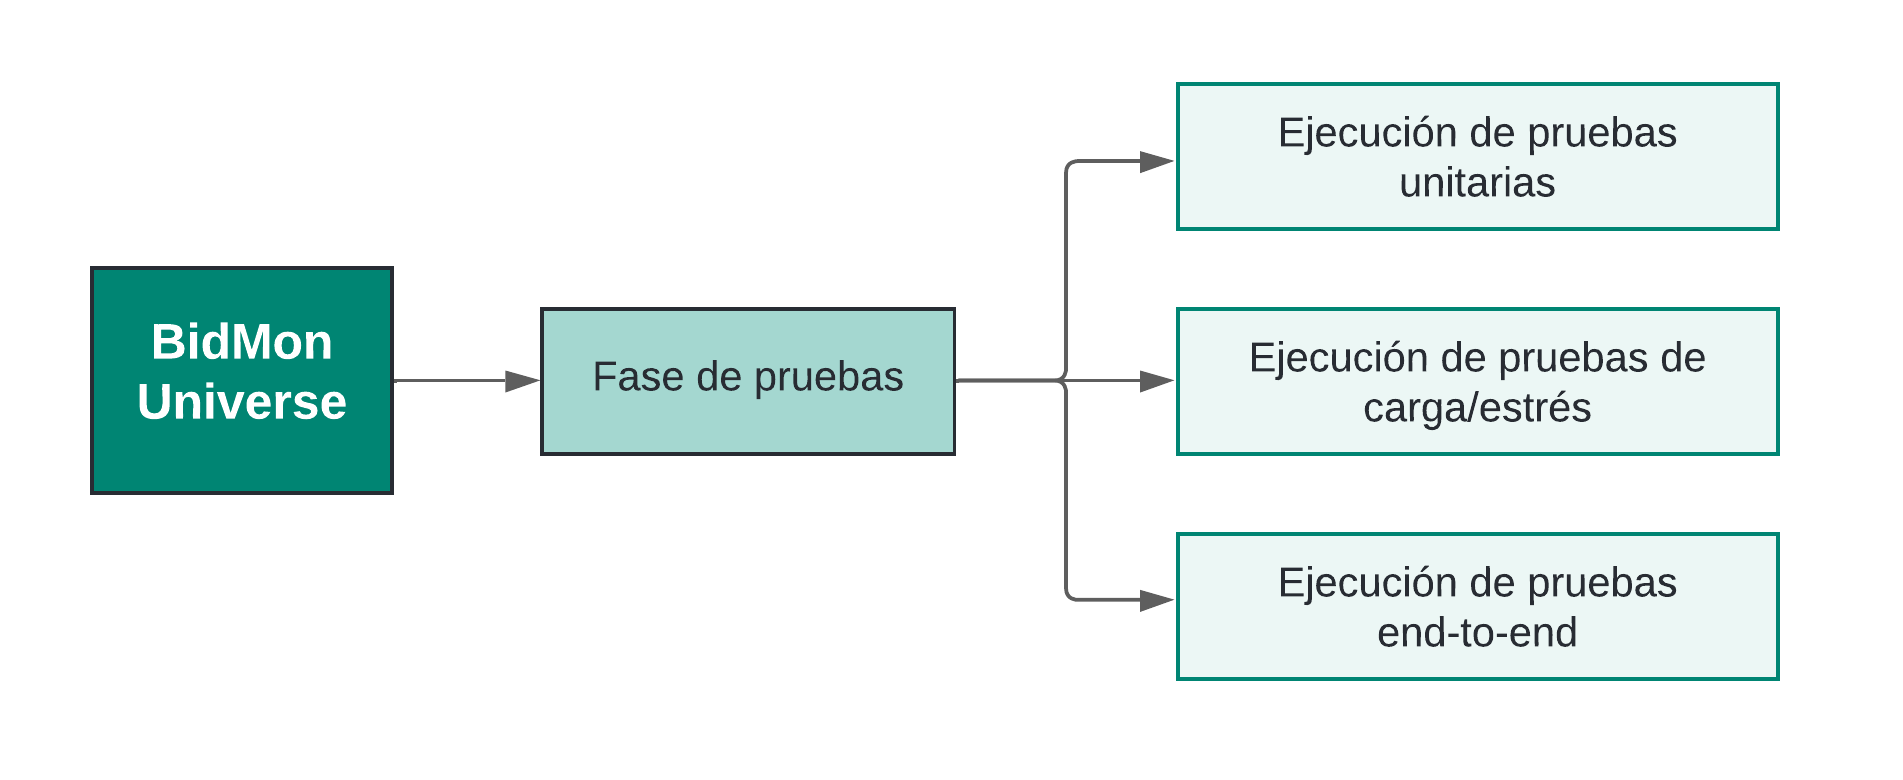
\includegraphics[width=0.9\linewidth]{figures/5-WBS/5_WBS-Pruebas.png}
    \caption{WBS. Fase de pruebas}
    \label{fig:5_WBS-Pruebas}
\end{figure}

\subsubsubsection{WBS. Despliegue del sistema}
En la fase de despliegue del sistema se realizan las tareas necesarias para poner en producción el sistema, como se detalla en la \coloredUnderline{\hyperlink{fig:5_WBS-Despliegue}{Figura \ref*{fig:5_WBS-Despliegue}: \nameref*{fig:5_WBS-Despliegue}}}.
\begin{figure}[H]
    \hypertarget{fig:5_WBS-Despliegue}{}
    \centering
    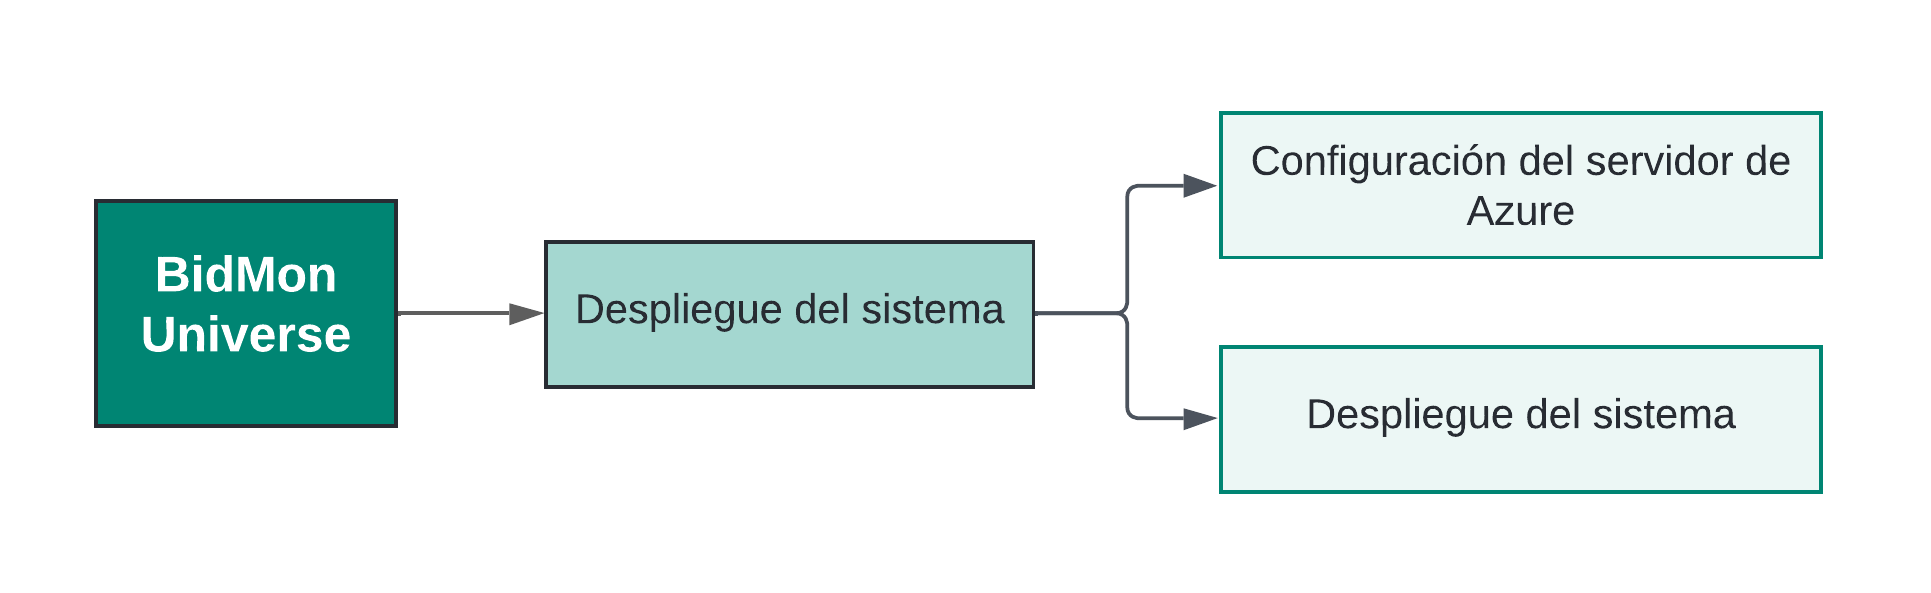
\includegraphics[width=0.9\linewidth]{figures/5-WBS/5_WBS-Despliegue2.png}
    \caption{WBS. Despliegue del sistema}
    \label{fig:5_WBS-Despliegue}
\end{figure}

\subsubsubsection{WBS. Documentación}
En la fase de documentación se realizan las tareas necesarias para la redacción de la memoria del proyecto, así como la preparación de la presentación del mismo.
\begin{figure}[H]
    \hypertarget{fig:5_WBS-Documentacion}{}
    \centering
    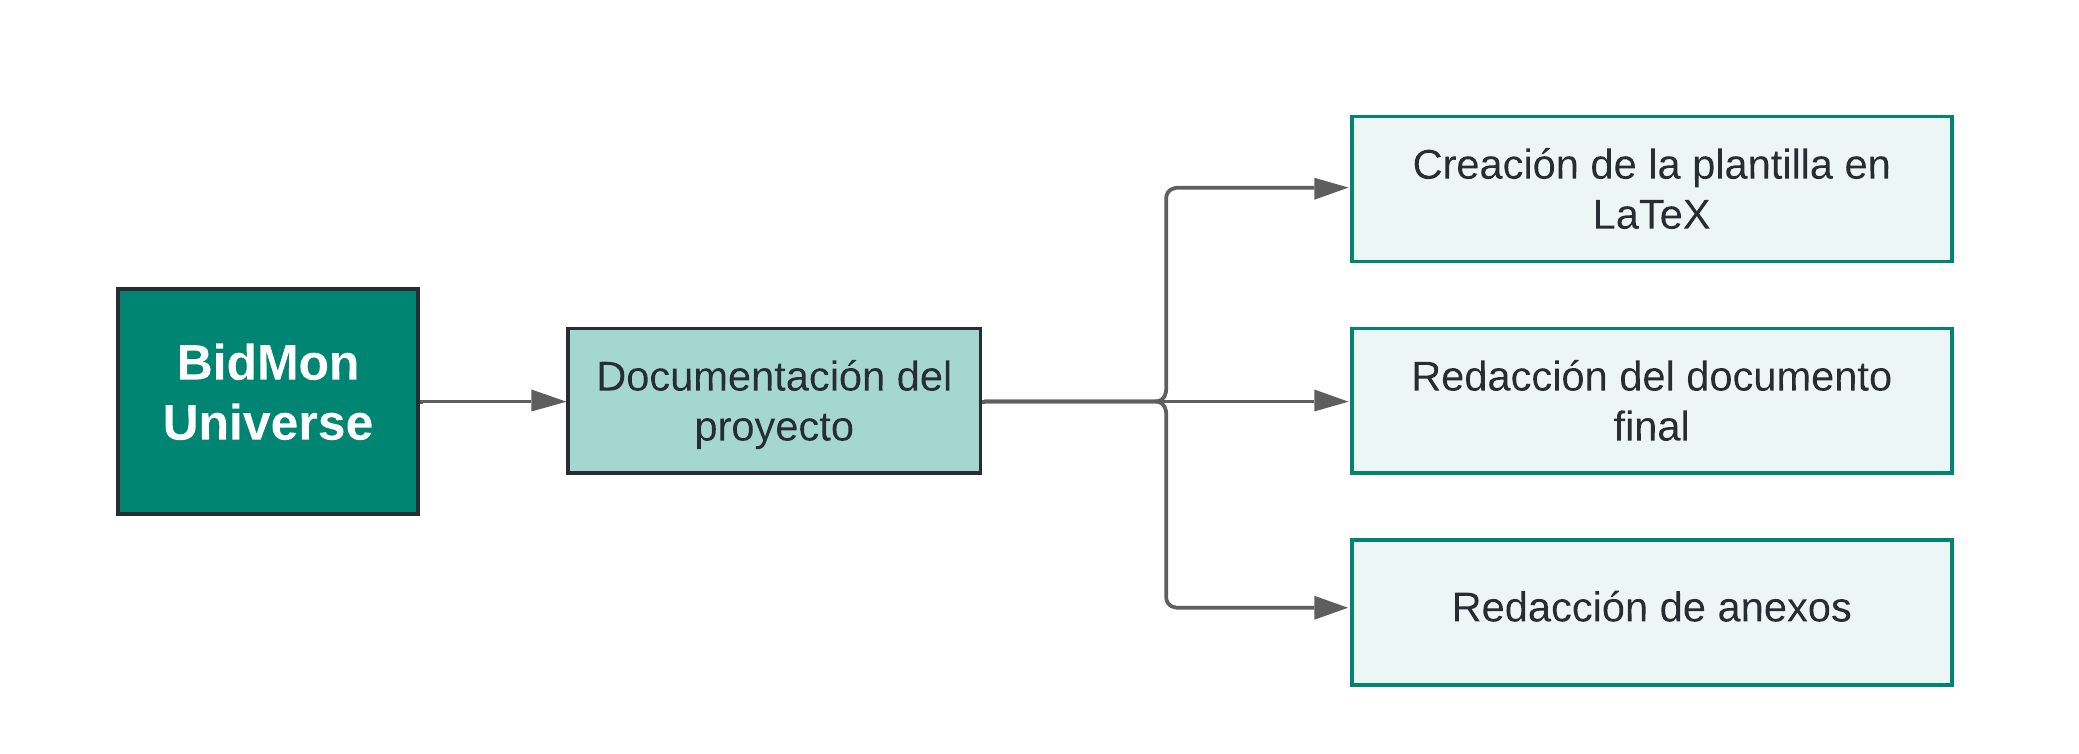
\includegraphics[width=0.9\linewidth]{figures/5-WBS/5_WBS-Documentacion.png}
    \caption{WBS. Documentación}
    \label{fig:5_WBS-Documentacion}
\end{figure}



\subsection{Riesgos}
\subsubsection{Plan de Gestión de Riesgos} 

\subsubsection{Identificación de Riesgos}


\subsubsection{Registro de Riesgos} 

\begin{table}[htb]
    \centering
    \caption{Análisis de riesgo}
    \label{table:risk_analysis}
    \begin{tabular}{>{\columncolor{rowcolor}}l l l}
    \toprule
    \rowcolor{lightgreen}
    \textbf{Identificador} & \multicolumn{2}{l}{1} \\
    \midrule
    \textbf{Nombre} & \multicolumn{2}{l}{Problema de costos} \\
    \midrule
    \textbf{Descripción} & \multicolumn{2}{p{10cm}}{El costo de desarrollar y mantener un sitio web y un sistema de venta y distribución es alto, lo que puede afectar negativamente la rentabilidad de la empresa si no se generan suficientes ingresos para cubrir estos costos.} \\
    \midrule
    \textbf{Categoría} & \multicolumn{2}{l}{Riesgo de gestión} \\
    \midrule
    \textbf{Probabilidad} & \multicolumn{2}{l}{Media} \\
    \midrule
    \textbf{Impacto} & Presupuesto & Crítico \\
    \cmidrule(lr){2-3}
    & Planificación & Medio \\
    \cmidrule(lr){2-3}
    & Alcance & Alto \\
    \cmidrule(lr){2-3}
    & Calidad & Alto \\
    \cmidrule(lr){2-3}
    & Total & 0.45 \\
    \midrule
    \textbf{Respuesta} & \multicolumn{2}{p{10cm}}{Realizar un análisis financiero riguroso para determinar el costo total del proyecto, incluyendo los costos de desarrollo, mantenimiento, actualizaciones y otros gastos asociados. Establecer proyecciones financieras realistas para garantizar que la empresa pueda generar suficientes ingresos para cubrir estos costos y obtener una rentabilidad adecuada.} \\
    \midrule
    \textbf{Estrategia} & \multicolumn{2}{l}{Mitigar el riesgo} \\
    \bottomrule
    \end{tabular}
    \end{table}





\subsection{Presupuesto Inicial}

\subsubsection{Presupuesto de Costes}

\subsubsection{Presupuesto de Cliente} 


\newpage
\section{EJECUCIÓN DEL PROYECTO}

\subsection{Plan Seguimiento de Planificación}

\subsection{Bitácora de Incidencias del Proyecto}

\subsection{Riesgos}


\newpage
\section{CIERRE DEL PROYECTO}

\subsection{Planificación Final}

\subsection{Informe Final de Riesgos}

\subsection{Presupuesto Final de Costes}



\subsection{Informe de Lecciones Aprendidas}

